% Official IEEE Transactions one-column template configuration (December 2023).
% Source: TITS_LaTeX_Template.zip, one-column.tex.
\documentclass[lettersize,onecolumn]{IEEEtran}
\usepackage{amsmath,amsfonts}
\usepackage{amssymb,amsthm,bm,mathtools}
\usepackage{algorithmic}
\usepackage{algorithm}
\usepackage{array}
\usepackage[caption=false,font=normalsize,labelfont=sf,textfont=sf]{subfig}
\usepackage{textcomp}
\usepackage{stfloats}
\usepackage{url}
\usepackage{verbatim}
\usepackage{graphicx}
\usepackage{float}
\usepackage{cite}
\usepackage{booktabs}
\usepackage{xcolor}
\usepackage[hidelinks]{hyperref}
\usepackage{orcidlink}
\usepackage{tikz}
\usetikzlibrary{arrows.meta,backgrounds,calc,fit,positioning}
\usepackage{pgfplots}
\pgfplotsset{compat=1.18}
\hyphenation{op-tical net-works semi-conduc-tor IEEE-Xplore}

\newtheorem{theorem}{Theorem}
\newtheorem{proposition}{Proposition}
\newtheorem{corollary}{Corollary}
\newtheorem{lemma}{Lemma}
\theoremstyle{remark}
\newtheorem{remark}{Remark}
\theoremstyle{definition}
\newtheorem{definition}{Definition}

\newcommand{\R}{\mathbb R}
\newcommand{\C}{\mathbb C}
\newcommand{\EE}{\mathbb E}
\newcommand{\PP}{\mathbb P}
\newcommand{\tr}{\operatorname{tr}}
\newcommand{\rank}{\operatorname{rank}}
\newcommand{\norm}[1]{\left\lVert #1\right\rVert}
\newcommand{\I}{\mathcal I}
\newcommand{\Lloss}{\mathcal L}
\newcommand{\Bbase}{\mathcal B}
\newcommand{\Pset}{\mathcal P_K}
\newcommand{\Stwo}{S_2}

% The manuscript figures are defined here so the full vector source stays in main.tex.
\newcommand{\ProjectiveSphereFigure}{%
\begin{figure}[t]
\centering
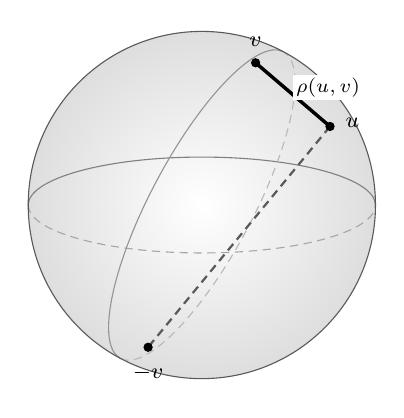
\begin{tikzpicture}[scale=1.05]
\coordinate (O) at (0,0);
\coordinate (U) at (1.55,0.95);
\coordinate (V) at (0.65,1.72);
\coordinate (Vm) at (-0.65,-1.72);
\shade[inner color=white,outer color=black!13] (O) circle (2.1);
\draw[black!35,densely dashed] (-2.1,0) arc[start angle=180,end angle=360,x radius=2.1,y radius=0.58];
\draw[black!50] (2.1,0) arc[start angle=0,end angle=180,x radius=2.1,y radius=0.58];
\draw[black!28,densely dashed,rotate=62] (-2.1,0) arc[start angle=180,end angle=360,x radius=2.1,y radius=0.62];
\draw[black!42,rotate=62] (2.1,0) arc[start angle=0,end angle=180,x radius=2.1,y radius=0.62];
\draw[black!65,densely dashed,line width=0.8pt] (U)--(Vm);
\draw[black,line width=1.25pt] (U)--(V);
\fill[black] (U) circle (1.6pt) (V) circle (1.6pt) (Vm) circle (1.6pt);
\draw[black!65] (O) circle (2.1);
\node[font=\footnotesize,anchor=west] at (1.62,1.0) {$u$};
\node[font=\footnotesize,anchor=south] at (0.65,1.80) {$v$};
\node[font=\footnotesize,anchor=north] at (-0.65,-1.82) {$-v$};
\node[font=\scriptsize,fill=white,inner sep=1pt,anchor=west] at (1.10,1.42) {$\rho(u,v)$};
\end{tikzpicture}
\caption{Projective geometry on the unit sphere. The solid chord joins $u$
to the closer representative $v$; the dashed chord joins $u$ to $-v$.
Because $vv^\top=(-v)(-v)^\top$, both endpoints represent the same
rank-one projector. The transport cost uses the shorter chord
$\rho(u,v)=\min\{\|u-v\|,\|u+v\|\}$.}
\label{fig:projective_quotient}
\end{figure}%
}

\newcommand{\OptimizerChartFigure}{%
\pgfmathdeclarefunction{chartcov}{3}{%
  \pgfmathparse{(cos(deg(##3-0.30932))+##1*sin(deg(##3-0.30932)))^2
  /(1+##1^2+##2^2)}%
}
\pgfmathdeclarefunction{chartinfo}{3}{%
  \pgfmathparse{(
    0.45*ln(1+##3*chartcov(##1,##2,0))
   +0.25*ln(1+##3*chartcov(##1,##2,0.6))
   +0.20*ln(1+##3*chartcov(##1,##2,1.3))
   +0.10*ln(1+##3*chartcov(##1,##2,2.2)))/2}%
}
\begin{figure}[H]
\centering
\begin{tikzpicture}
\begin{axis}[
  width=0.76\textwidth,height=7.0cm,view={53}{29},
  xlabel={$t$},ylabel={$s$},zlabel={millinats},
  xlabel style={font=\footnotesize},ylabel style={font=\footnotesize},
  zlabel style={font=\footnotesize},tick label style={font=\scriptsize},
  xmin=-0.10,xmax=0.14,ymin=-0.15,ymax=0.15,
  xtick={-0.10,0,0.05,0.10},ytick={-0.15,0,0.15},
  zmin=-13,zmax=1,ztick={-12,-6,0},
  grid=major,grid style={black!12},
  colormap={papergray}{gray(0cm)=(0.92); gray(1cm)=(0.28)},
  point meta min=-13,point meta max=1,
]
\addplot3[surf,shader=interp,draw=black!20,opacity=0.94,
  samples=25,samples y=25,domain=-0.10:0.14,y domain=-0.15:0.15]
  {1000*(chartinfo(x,y,3)-chartinfo(0,0,3))};
\addplot3[black,only marks,mark=o,mark size=2.1pt]
  coordinates {(0,0,0)};
\addplot3[black,only marks,mark=*,mark size=2.0pt]
  coordinates {(0.04858,0,0.6108)};
\node[font=\scriptsize,fill=white,inner sep=1pt]
  at (axis cs:0.005,-0.02,0.7) {$P_0$};
\node[font=\scriptsize,fill=white,inner sep=1pt]
  at (axis cs:0.078,0.002,0.8) {$P_3$};
\end{axis}
\end{tikzpicture}
\caption{Local three-dimensional information landscape for the four-direction
law of Fig.~\ref{fig:stability}, embedded in $\mathbb R^3$ at SNR $\gamma=3$.
Height is $10^3[\I_\mu(P_{v(t,s)};3)-\I_\mu(P_0;3)]$ in millinats.
The open dot is the covariance projector $P_0$; the filled dot is the
numerically selected information maximizer $P_3$ at $t\approx0.04858$,
$s=0$. This local plot illustrates optimizer displacement; it does not
certify the global maximum.}
\label{fig:optimizer_chart_3d}
\end{figure}%
}

% Generated by scripts/reproduce.py
\newcommand{\KSReal}{4.86\times10^{-3}}
\newcommand{\KSComplex}{5.32\times10^{-3}}
\newcommand{\SlopeAxes}{1.998}
\newcommand{\SlopeIcosa}{2.996}
\newcommand{\ACGInfo}{1.9726}
\newcommand{\ACGSE}{0.0018}
\newcommand{\ACGBound}{2.0557}
\newcommand{\HaarTwenty}{1.4483}
\newcommand{\BPSKRatio}{0.4565}
\newcommand{\BPSKError}{3.33\times10^{-16}}
\newcommand{\MomentError}{2.50\times10^{-16}}

% Generated by scripts/reproduce_core.py
\newcommand{\CoreGap}{0.41548}
\newcommand{\CoreAngle}{0.30932}
\newcommand{\CoreA}{-0.030791}
\newcommand{\CoreTilt}{0.074109}
\newcommand{\CoreDistanceLimit}{0.104806}
\newcommand{\CoreRegretLimit}{1.14\times10^{-3}}
\newcommand{\CoreDistanceSlope}{0.999}
\newcommand{\CoreRegretSlope}{2.996}
\newcommand{\CoreMomentResidual}{1.22\times10^{-15}}
\newcommand{\CoreCompressionError}{7.43\times10^{-6}}
\newcommand{\CoreCompressionRegret}{1.61\times10^{-9}}
\newcommand{\CoreEmpiricalErrorA}{1.42\times10^{-2}}
\newcommand{\CoreEmpiricalErrorB}{7.14\times10^{-3}}
\newcommand{\CoreEmpiricalErrorC}{3.56\times10^{-3}}
\newcommand{\CoreEmpiricalErrorD}{1.82\times10^{-3}}
\newcommand{\CoreEmpiricalSlope}{-0.495}

% Generated by reproduce_rank.py
\newcommand{\RankError}{5.13\times10^{-3}}
\newcommand{\RankRegret}{2.02\times10^{-4}}
\newcommand{\RankResidual}{6.66\times10^{-16}}
\newcommand{\RankCandidates}{525}

\begin{document}

\title{Stability of Information-Optimal Fixed Subspace Measurements Under Directional Uncertainty}

\author{Huy Hoang Le\,\orcidlink{0009-0009-2138-5468} and Kim-Anh Nguyen\,\orcidlink{0000-0003-3408-847X}%
\thanks{Huy Hoang Le is with the Research and Development Department, PowerMore Ltd., Da Nang 550000, Viet Nam (e-mail: lhhoang@powermore.vn).}%
\thanks{Kim-Anh Nguyen is with the Faculty of Electrical Engineering, University of Science and Technology, The University of Danang, Da Nang 550000, Viet Nam (e-mail: nkanh@dut.udn.vn).}%
\thanks{Corresponding author: Kim-Anh Nguyen.}}

\markboth{MANUSCRIPT FOR IEEE TRANSACTIONS ON INFORMATION THEORY}%
{Le and Nguyen: Stability of Information-Optimal Fixed Subspace Measurements}

\maketitle

\begin{abstract}
We study fixed subspace measurements of a random rank-one signal whose direction is available to the decoder. Retained information is a scalar additive white Gaussian noise channel information function averaged over the projection energy. We quantify the stability of information-optimal measurements under changes in signal-to-noise ratio (SNR) and in the directional law. Under a strict eigengap of the directional second moment, an explicit finite-SNR bound controls the distance of every global optimizer from the leading eigenspace and the information lost by using that eigenspace. Fourth-degree moments determine the first subspace displacement, whereas they can select the leading orientation when the second moment is isotropic. Moment matching and projective-Wasserstein perturbations control objective error and transferred-design regret; under quadratic growth, these bounds also control optimizer distance. A joint bound handles simultaneous SNR and directional-law mismatch. From finitely many observed directions, a uniform concentration bound holds over all projectors of the prescribed rank, and the empirical law can be compressed to a weighted moment-matching surrogate with an explicit high-probability information and design-regret guarantee. For Gaussian input, the compression error converges geometrically in the matching order at each finite SNR. A rotationally invariant directional benchmark and a covariance upper envelope are sharp over their respective classes of laws.
\end{abstract}

\begin{IEEEkeywords}
Mutual information, subspace measurements, directional uncertainty, projective Wasserstein distance, directional moments, cubature.
\end{IEEEkeywords}

\section{Introduction}
\IEEEPARstart{A}{ fixed} low-dimensional front end can preserve only part of a signal whose spatial direction changes after the measurement subspace has been chosen. We study this loss for a single scalar information-bearing amplitude multiplied by a random unit direction. The direction is known to the decoder. The model describes a coherent rank-one channel with a subspace combiner that is fixed over the directional ensemble. It isolates the effect of subspace restriction from channel estimation and hardware constraints.

Mutual-information expansions at low signal-to-noise ratio (SNR) are classical. Prelov and Verd\'u derived second-order asymptotics for multidimensional Gaussian-noise channels with general inputs and random parameters \cite{prelov2004}; their operational relevance in the wideband regime is developed in \cite{verdu2002}. The mutual-information--minimum-mean-square-error (I-MMSE) relation \cite{guo2005}, minimum mean-square error (MMSE) regularity and derivative formulas \cite{guo2011}, and mutual-information gradients and Hessians \cite{palomar2006,payaro2009} supply the analytic tools used here. Averaging a scalar information function over random channel gains is also standard in coherent fading with arbitrary inputs \cite{ramos2014}. Our contribution concerns the measurement subspace that generates those gains: quantitative stability of its optimizer under SNR and law perturbations, and finite-data representations that approximate the entire family of subspace objectives.

Carson \emph{et al.} develop information-based projection design for general signal priors, including mutual-information gradients and mode-exposure and mode-alignment structure \cite{carson2013}. Wang \emph{et al.} study a metric balancing classification and recovery, with Gaussian and Poisson measurement models, energy and orthonormality constraints, and structural characterizations of the solutions \cite{wang2017}. These works establish a broader design setting than the coherent rank-one model studied here. Go and Isaac address prior sensitivity of expected information gain through a Kullback--Leibler ambiguity-set formulation \cite{goisaac2022}. Our rank-one directional structure instead yields uniform projector-wise approximation, transferred-design regret, optimizer-distance bounds, and exact finite moment-preserving representations. Gradient and stationary-point characterizations alone do not supply this guarantee chain: the arguments below additionally use a scalar derivative envelope, an eigengap inequality, and uniform approximation over projector space.

Related Gaussian projection and information-bottleneck problems lead to covariance-defined representations \cite{giraldi2018,chechik2005}. Li, Baptista, and Marzouk study expected-information-gain estimation and gradient-based dimension reduction for parameters or observations \cite{li2026}. Our focus is a fixed-rank projector for a random rank-one direction and an explicit stability hierarchy through finite SNR, law replacement, optimizer transfer, and finite directional data. Fourth-degree directional structure then quantifies the first departure from covariance design even with a Gaussian scalar amplitude.

The geometry of random projections and subspace codebooks is established \cite{lu2007,kang2024,love2003,dai2008}. Grassmann quantization approximates subspaces by codewords; our directional surrogate instead replaces a probability law while retaining uniform control over the measurement objectives. We use the classical random-projection law as a universal information benchmark. Spherical designs reproduce polynomial moments \cite{delsarte1977,reznick1995}; because projection energy is even in the direction, projective designs and even-polynomial cubature are the relevant underlying objects \cite{hughes2021}. Positive finite cubature follows from Tchakaloff's theorem \cite{bayer2006}. We explicitly credit these existence results and use them to obtain information-error and design-transfer guarantees with a support-size bound for arbitrary directional laws.

The distinction between a Haar-uniform law, meaning the rotation-invariant uniform law, and a law with isotropic second moment is essential. A finite ensemble can have a second moment proportional to the identity and still prefer specific measurement orientations. We quantify this distinction using coverage moments and give examples with equal second moments but different optimal subspaces.

We use $\R^d$ for real Euclidean space of dimension $d$, $v^{\top}$ for transpose, $\EE$ for expectation, and $I(X;Y)$ and $I(X;Y\mid V)$ for mutual information and conditional mutual information, respectively. Let $d\ge2$ be the observation dimension and $1\le K<d$ the measurement rank. We formalize the problem through the scalar-mode model
\begin{equation}
Y=\sqrt{\gamma}\,UR+N,
\label{eq:intro_model}
\end{equation}
where $Y\in\R^d$ is the observation, $R$ is a scalar amplitude with unit variance, $U\in\R^d$ is a random unit direction with law $\mu$, $N$ is independent standard Gaussian noise, and $\gamma\ge0$ is the SNR. The rank-$K$ orthogonal measurement projector $P$ is fixed before $U$ is realized. The receiver is given $U$ in the conditional information criterion considered here. Conditioned on $U=u$, only the squared projection
\begin{equation}
C_P(u)=u^{\top}Pu
\end{equation}
reaches the measurement space. Let $h_R(s)=I(R;\sqrt{s}R+Z_0)$ denote the scalar additive white Gaussian
noise (AWGN) mutual information at SNR $s\ge0$, where $Z_0$ is a standard
real Gaussian variable independent of $R$. Then the high-dimensional problem
reduces exactly to the scalar functional
\begin{equation}
\I_\mu(P;\gamma)=\EE_{U\sim\mu}\!\left[h_R\!\left(\gamma C_P(U)\right)\right],
\label{eq:intro_functional}
\end{equation}
where the notation $U\sim\mu$ means that $U$ has probability law $\mu$.

The central question is how stable an information-optimal fixed measurement remains when the SNR or the directional law is uncertain. Three main results organize the answer at the measurement, information-limit, and statistical-representation levels.
\begin{enumerate}
\item \emph{Stability of covariance-based measurement.} Theorem~\ref{thm:stability} combines finite-SNR distance and information-regret certificates with the low-SNR optimal-value expansion. The second moment selects the limiting subspace; fourth-degree contractions determine its first departure and the cubic information cost in Corollary~\ref{cor:cubic_regret}. Under an isotropic second moment, fourth-degree geometry can instead select the leading orientation (Corollary~\ref{cor:fourth}).
\item \emph{Sharp information benchmarks.} Theorem~\ref{thm:sandwich} combines a universal Haar lower benchmark and a covariance upper envelope with their attainability statements. It specifies what can be guaranteed across directional laws and what a prescribed second moment alone can determine.
\item \emph{Directional-law stability and finite representation.} Theorem~\ref{thm:representation} gives moment-based objective, optimal-value, and design-transfer bounds and a finite weighted surrogate valid at every rank. Proposition~\ref{prop:wasserstein} gives a direct projective-Wasserstein perturbation bound. Under quadratic growth, Corollary~\ref{cor:law_optimizer} converts uniform objective error into optimizer distance, while Corollary~\ref{cor:joint_perturbation} gives joint SNR--directional-law stability. Corollary~\ref{cor:finite_sample} carries the chain from observed directions through empirical-law compression to high-probability information and design-regret guarantees.
\end{enumerate}

The novelty is the guarantee chain within one coverage functional: the second moment specifies the covariance design, SNR perturbation moves its optimizer according to fourth-order geometry, law perturbation controls objectives and transferred designs, uniform objective error controls optimizer distance, and finite samples lead to a compressed directional representation. The outputs are quantified directly in mutual-information units through information loss, design-transfer regret, and the geometry of information-optimal measurements, rather than only through perturbation of a generic optimization objective. Scalar reduction, Taylor expansion, spectral-gap arguments, concentration, transport bounds, and positive cubature are supporting tools. The support bound can grow rapidly with dimension and matching order, and it does not promise efficient construction or global measurement optimization.

The remainder is organized as follows. Section~II defines the model and coverage functional. Section~III establishes covariance-design stability and its fourth-order geometry. Section~IV gives the sharp information sandwich. Section~V develops statistical stability and finite directional representations. Section~VI gives exact Gaussian reference laws. Section~VII reports theory-driven experiments. Sections~VIII and IX discuss scope and conclude.

\section{Problem Formulation and Coverage Geometry}

The identity matrix of size $m$ is $I_m$, and $e_i$ is the $i$th standard basis vector. We write $\|v\|$ for the Euclidean norm, $\|A\|_F=(\sum_{i,j}|A_{ij}|^2)^{1/2}$ for the Frobenius norm, and $\|A\|_{\rm op}=\sup_{\|v\|=1}\|Av\|$ for the operator norm. The symbols $\tr A$, $\rank A$, and $\operatorname{diag}(a_1,\ldots,a_m)$ denote trace, rank, and the diagonal matrix with the displayed entries. The unit sphere is $\mathbb S^{d-1}=\{u\in\R^d:\|u\|=1\}$. We write $\mathcal N(m,\Sigma)$ for the real Gaussian distribution with mean $m$ and covariance $\Sigma$, and $X\perp Y$ for independence.

Let $P_R$ be the law of the amplitude $R$, and assume
\begin{equation}
\begin{gathered}
R\sim P_R, \qquad \EE[R]=0, \qquad \EE[R^2]=1,\qquad R\perp U,\\
U\sim\mu,\qquad \mu\text{ a probability law on }\mathbb S^{d-1}.
\end{gathered}
\label{eq:model}
\end{equation}
The observation is
\begin{equation}
Y=\sqrt{\gamma}\,UR+N,
\qquad N\sim\mathcal N(0,I_d),
\end{equation}
where $N$ is independent of $(R,U)$ and $\gamma\ge0$. Throughout, $d\ge2$ and $1\le K<d$; the endpoints $K=0$ and $K=d$ give zero and full information, respectively. All logarithms are natural and information is measured in nats. Let $\Pset$ denote the set of rank-$K$ orthogonal projectors on $\R^d$. A fixed rank-$K$ linear front end is represented by
\begin{equation}
P=P^{\top}=P^2, \qquad \tr P=K,
\qquad P\in\Pset.
\end{equation}
Write $Z=W^{\top}Y$, where $W\in\R^{d\times K}$ satisfies $W^{\top}W=I_K$ and $WW^{\top}=P$. Every full-row-rank measurement matrix $A\in\R^{K\times d}$ is equivalent to this representation: whitening $AY$ by $(AA^{\top})^{-1/2}$ is invertible and produces an orthonormal-row measurement with the same row space. Thus the projector formulation includes arbitrary noiseless linear processing of $Y$ of rank $K$; it does not include additional measurement noise or quantization.

The measurement is chosen from the known or estimated law $\mu$ before $U$ is realized. The decoder is supplied with $U$ as ideal side information, for example by a separate training stage whose cost is outside the model. The uncertainty is therefore pre-measurement design uncertainty, rather than receiver-side channel-state uncertainty: the fixed front end is selected before the realization of $U$, whereas the decoder knows $U$ after measurement. We do not assume that $U$ can itself be recovered from the compressed observation. Consequently, the objective measures subspace loss in a coherent channel, rather than information about a hidden direction or a general multi-stream signal.

\subsection{Coverage Reduction}
Define the coverage
\begin{equation}
C_P(u)=u^{\top}Pu=\norm{W^{\top}u}^2\in[0,1].
\label{eq:coverage}
\end{equation}
Figure~\ref{fig:projection_geometry} shows the rank-two case in three
dimensions. Write $\mathcal S=\operatorname{range}(P)$ for the fixed
measurement plane. Only the component in $\mathcal S$ contributes to
coverage; the orthogonal residual contributes no conditional information.
\begin{figure}[H]
\centering
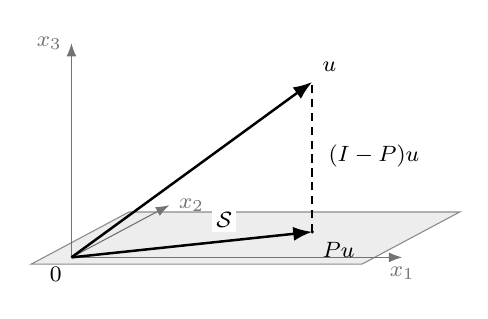
\begin{tikzpicture}[
  x={(3.5cm,0cm)},y={(1.35cm,0.72cm)},z={(0cm,3.4cm)},
  >=Latex,font=\footnotesize,
  vec/.style={-{Latex[length=2.4mm]},line width=0.9pt},
  guide/.style={densely dashed,line width=0.65pt}
]
  \coordinate (O) at (0,0,0);
  \coordinate (Q) at (0.70,0.45,0);
  \coordinate (U) at (0.70,0.45,0.56);
  \fill[black!7] (-0.10,-0.12,0) -- (1.10,-0.12,0) --
    (1.10,0.80,0) -- (-0.10,0.80,0) -- cycle;
  \draw[black!45] (-0.10,-0.12,0) -- (1.10,-0.12,0) --
    (1.10,0.80,0) -- (-0.10,0.80,0) -- cycle;
  \draw[->,black!55] (O) -- (1.20,0,0) node[below] {$x_1$};
  \draw[->,black!55] (O) -- (0,0.92,0) node[right] {$x_2$};
  \draw[->,black!55] (O) -- (0,0,0.80) node[left] {$x_3$};
  \draw[vec] (O) -- (U) node[above right] {$u$};
  \draw[vec] (O) -- (Q) node[below right] {$Pu$};
  \draw[guide] (Q) -- (U);
  \fill (Q) circle[radius=0.65pt];
  \node[right] at (0.72,0.46,0.28) {$(I-P)u$};
  \node[fill=white,inner sep=1.5pt] at (0.30,0.66,0) {$\mathcal S$};
  \node[below left] at (O) {$0$};
\end{tikzpicture}
\caption{Orthogonal projection onto a fixed rank-two measurement plane.
The retained energy is $C_P(u)=\|Pu\|^2$; the dashed residual
$(I-P)u$ is orthogonal to the plane. The picture illustrates the coverage
functional and does not assume that the receiver must estimate $u$.}
\label{fig:projection_geometry}
\end{figure}
For the scalar AWGN information function
\begin{equation}
h_R(s)=I\!\left(R;\sqrt{s}R+Z_0\right),
\qquad Z_0\sim\mathcal N(0,1),
\label{eq:h}
\end{equation}
with $Z_0$ independent of $R$, we define the conditional fixed-measurement information
\begin{equation}
\I_\mu(P;\gamma)
\triangleq I(R;Z\mid U)
=
\EE_{U\sim\mu}\left[h_R\!\left(\gamma C_P(U)\right)\right].
\label{eq:core_functional}
\end{equation}
The superscript $\star$ denotes optimization over $\Pset$:
\begin{equation}
\I_\mu^\star(\gamma)=\max_{P\in\Pset}\I_\mu(P;\gamma).
\end{equation}
It exists by compactness of $\Pset$ and continuity of the bounded integrand. Full observation gives $I(R;Y\mid U)=h_R(\gamma)$, so the information loss $\Lloss_\mu$ and its minimum $\Lloss_\mu^\star$ are
\begin{equation}
\begin{aligned}
\Lloss_\mu(P;\gamma)&\triangleq h_R(\gamma)-\I_\mu(P;\gamma),\\
\Lloss_\mu^\star(\gamma)&\triangleq h_R(\gamma)-\I_\mu^\star(\gamma).
\end{aligned}
\label{eq:loss_definition}
\end{equation}

\begin{lemma}[Coverage reduction]\label{lem:reduction}
For every $P\in\Pset$ and every $u\in\mathbb S^{d-1}$, the conditional mutual information of the $K$-dimensional measurement equals the scalar AWGN information at SNR $\gamma C_P(u)$.
\end{lemma}
\begin{proof}
Let $a=W^{\top}u$. If $a=0$, the measurement contains noise independent of $R$. Otherwise, rotate the $K$-dimensional measurement by an orthogonal matrix whose first row is $a^{\top}/\norm a$. The first rotated coordinate equals $\sqrt{\gamma}\norm a R+Z_1$, where $Z_1$ is independent standard real Gaussian noise, whereas the remaining coordinates contain only Gaussian noise independent of $R$. Thus the conditional information equals $h_R(\gamma\norm a^2)=h_R(\gamma C_P(u))$.
\end{proof}

For Gaussian $R\sim\mathcal N(0,1)$,
\begin{equation}
h_R(s)=\frac12\log(1+s).
\label{eq:gaussian_h}
\end{equation}
No Gaussian assumption is needed for Lemma~\ref{lem:reduction}. By the I-MMSE relation, $h_R$ is nondecreasing and concave for the finite-variance scalar Gaussian channel \cite{guo2005}.

Smoothness at zero is stated separately in the results that need it; finite variance alone is not used to justify arbitrary-order differentiation. Bounded inputs and Gaussian inputs satisfy the finite-order regularity used below. The MMSE derivative identities \cite{guo2011} give $h_R'(0)=1/2$ and $h_R''(0)=-1/2$ for centered unit-variance inputs when the corresponding right derivatives extend continuously to zero. Thus the first two coefficients apply, in particular, to every bounded constellation as well as to Gaussian signaling.

\subsection{Coverage Moments and Directional Moments}
Define the coverage moments
\begin{equation}
M_n(P;\mu)=\EE_\mu\left[C_P(U)^n\right],
\qquad n\ge1,
\label{eq:Mn}
\end{equation}
and the second-order directional moment matrix
\begin{equation}
S_2=\EE[UU^{\top}].
\label{eq:S2}
\end{equation}
This is the uncentered directional moment. It is also the covariance of the signal $UR$, since $R$ is independent of $U$ and has zero mean and unit variance; no assumption on $\EE U$ is needed.
Then
\begin{equation}
M_1(P;\mu)=\tr(PS_2).
\label{eq:M1}
\end{equation}
Let $\lambda_i(S_2)$ denote the eigenvalues of $S_2$ in nonincreasing order, and define
\begin{equation}
a_K(S_2)=\sum_{i=1}^{K}\lambda_i(S_2),
\qquad \lambda_1\ge\cdots\ge\lambda_d.
\label{eq:aK}
\end{equation}

\begin{remark}
The matrix $S_2$ contains all second-order directional information. It does not, in general, determine $M_n$ for $n\ge2$. This distinction is the source of the higher-order information hierarchy studied below.
\end{remark}

\section{SNR Stability of Covariance-Based Measurement}

\subsection{Uniform Finite-Order Expansion}
The central expansion is finite-order rather than an unrestricted infinite Taylor series. Here $r\ge1$ is an integer expansion order and $\gamma_0>0$ is an SNR endpoint. The notation $C^m([0,\gamma_0])$ denotes functions with $m$ continuous derivatives, with one-sided derivatives at the endpoints; $h_R^{(n)}$ is the $n$th derivative. As $\gamma\downarrow0$, $f=O(g)$ means $|f|\le c|g|$ for a fixed constant $c$ at sufficiently small positive $\gamma$, and $f=o(g)$ means $f/g\to0$. For nonnegative quantities, $f=\Theta(g)$ means that $f/g$ is bounded above and below by positive constants. Matrix versions use the Frobenius norm.

\begin{lemma}[Uniform coverage-moment expansion]\label{lem:expansion}
Suppose $h_R\in C^{r+1}([0,\gamma_0])$. Define
\begin{equation}
b_n=\frac{h_R^{(n)}(0)}{n!},\qquad n=1,\ldots,r.
\end{equation}
Then, for every $0\le\gamma\le\gamma_0$,
\begin{equation}
\I_\mu(P;\gamma)
=\sum_{n=1}^{r}b_n\gamma^nM_n(P;\mu)+R_{r+1}(P,\gamma),
\label{eq:finite_expansion}
\end{equation}
with the uniform remainder bound
\begin{equation}
\sup_{P\in\Pset}|R_{r+1}(P,\gamma)|
\le
\frac{\gamma^{r+1}}{(r+1)!}
\sup_{0\le s\le\gamma}|h_R^{(r+1)}(s)|.
\label{eq:remainder}
\end{equation}
Hence the coefficient of $\gamma^n$ is $b_n$ times the $n$th coverage moment, and $C_P(u)^n=(u^{\top}Pu)^n$ is a polynomial of degree $2n$ in $u$.
\end{lemma}
\begin{proof}
Taylor's theorem gives
\begin{equation*}
h_R(\gamma c)=\sum_{n=1}^{r}b_n(\gamma c)^n+\rho_{r+1}(c),
\end{equation*}
where
\begin{equation*}
|\rho_{r+1}(c)|\le\frac{(\gamma c)^{r+1}}{(r+1)!}\sup_{0\le s\le\gamma}|h_R^{(r+1)}(s)|.
\end{equation*}
Because $0\le c\le1$, the displayed upper bound is uniform in $c$ and therefore in $P$ and $U$. Taking expectation yields \eqref{eq:finite_expansion} and \eqref{eq:remainder}.
\end{proof}

For Gaussian input, the first three terms are
\begin{equation}
\I_\mu(P;\gamma)
=\frac{\gamma}{2}M_1(P;\mu)-\frac{\gamma^2}{4}M_2(P;\mu)+\frac{\gamma^3}{6}M_3(P;\mu)+R_4.
\label{eq:gaussian_series}
\end{equation}
More generally, for any fixed $r$, the finite-order formula is valid without requiring $\gamma<1$.

\subsection{Main Stability Theorem}
Let $P_0$ be the projector onto the leading $K$ eigenvectors of $S_2$. The next theorem gives both finite-SNR guarantees and, under additional regularity, the low-SNR expansion for every global optimizer.

\begin{theorem}[Stability of covariance-based measurement]\label{thm:stability}
Suppose $h_R\in C^1([0,\gamma_0])$ for some $\gamma_0>0$, $a=h_R'(0)>0$, and $\Delta=\lambda_K(S_2)-\lambda_{K+1}(S_2)>0$. Set
\begin{equation}
\beta_\gamma=\sup_{0\le s\le\gamma}|h_R'(s)-a|.
\end{equation}
\emph{(a) Finite-SNR certificate.} For every $0<\gamma\le\gamma_0$ and every global optimizer $P_\gamma$,
\begin{align}
\|P_\gamma-P_0\|_F&\le\frac{\sqrt2\,\beta_\gamma}{a\Delta},\label{eq:explicit_distance}\\
0\le\I_\mu^\star(\gamma)-\I_\mu(P_0;\gamma)
&\le\frac{\gamma\beta_\gamma^2}{4a\Delta}.\label{eq:explicit_regret}
\end{align}
If additionally $h_R\in C^2([0,\gamma_0])$ and $\sup_{[0,\gamma]}|h_R''|\le L$, these bounds are respectively $\sqrt2 L\gamma/(a\Delta)$ and $L^2\gamma^3/(4a\Delta)$. Under this $C^2$ assumption, $\I_\mu^\star(\gamma)=a\,a_K(S_2)\gamma+O(\gamma^2)$. For Gaussian input the distance and regret bounds become
\begin{align}
\|P_\gamma-P_0\|_F&\le\frac{\sqrt2\gamma}{(1+\gamma)\Delta},\\
\I_\mu^\star(\gamma)-\I_\mu(P_0;\gamma)&\le\frac{\gamma^3}{8(1+\gamma)^2\Delta}.
\label{eq:gauss_regret}
\end{align}
In particular, $P_\gamma\to P_0$ as $\gamma\downarrow0$.

\emph{(b) Low-SNR expansion.} If additionally $h_R\in C^3([0,\gamma_0])$, then
\begin{equation}
\I_\mu^\star(\gamma)=h_R'(0)a_K(S_2)\gamma
+\tfrac12h_R''(0)M_2(P_0;\mu)\gamma^2+O(\gamma^3),
\label{eq:second_opt}
\end{equation}
and $\|P_\gamma-P_0\|_F=O(\gamma)$ for every optimizer.
\end{theorem}
\begin{proof}
\emph{(a)} Let $D=\|P-P_0\|_F$. The spectral-gap inequality is
\begin{equation}
\tr((P_0-P)S_2)\ge\Delta(K-\tr(PP_0))=\frac{\Delta D^2}{2}.
\label{eq:gap_distance}
\end{equation}
Indeed, in an eigenbasis of $S_2$, the trace loss is at least $\Delta$ times the mass that $P$ places outside the leading eigenspace. For equal-rank orthogonal projectors, the nonzero eigenvalues of $P-P_0$ occur in opposite pairs (the sines of the principal angles); hence $\|P-P_0\|_{\rm op}\le D/\sqrt2$.

Write $g_\gamma(c)=h_R(\gamma c)-a\gamma c$. Since $|g_\gamma'(c)|\le\gamma\beta_\gamma$ on $[0,1]$,
\begin{equation}
\I_\mu(P;\gamma)-\I_\mu(P_0;\gamma)
\le-\frac{a\gamma\Delta D^2}{2}
+\frac{\gamma\beta_\gamma D}{\sqrt2}.
\label{eq:quadratic_tradeoff}
\end{equation}
For $P=P_\gamma$ the left side is nonnegative; dividing by $D$ when $D>0$ proves \eqref{eq:explicit_distance}. Maximizing the quadratic right side over $D\ge0$ proves \eqref{eq:explicit_regret}. The curvature estimate follows from the mean-value theorem. In the Gaussian case $a=1/2$ and $\beta_\gamma=\gamma/[2(1+\gamma)]$.
Continuity of $h_R'$ at zero makes $\beta_\gamma\to0$, proving convergence to $P_0$. Under the stated $C^2$ assumption, the uniform first-order expansion in Lemma~\ref{lem:expansion} and maximization of $\tr(PS_2)$ give the first-order value formula.

\emph{(b)} Appendix~\ref{app:subspace} applies the implicit-function theorem to the gradient of the normalized objective in a local chart. Part (a) places every global optimizer near $P_0$ for sufficiently small SNR, so each lies on the resulting stationary branch. The displacement is $O(\gamma)$, the leading trace changes quadratically, and evaluation of the second-order coefficient at $P_0$ gives \eqref{eq:second_opt}.
\end{proof}

The bounds can be loose when $\Delta$ is small and do not assert finite-SNR uniqueness. Their value is an explicit certificate for using $P_0$. For example, in the Gaussian case and any prescribed $0<\epsilon<\sqrt2$, the condition
$\gamma\le\epsilon\Delta/(\sqrt2-\epsilon\Delta)$ guarantees $\|P_\gamma-P_0\|_F\le\epsilon$.

\begin{corollary}[Cubic cost of covariance-only design]\label{cor:cubic_regret}
Under the $C^3$ hypotheses of Theorem~\ref{thm:stability}(b), write $U=(x^{\top},y^{\top})^{\top}$ in an orthonormal eigenbasis of $S_2$, where $x\in\R^K$ contains the leading coordinates and $y\in\R^{d-K}$ the remaining coordinates. Define $A_{ji}=\EE[\|x\|^2y_jx_i]$; Appendix~\ref{app:subspace} gives the corresponding local chart. Then
\begin{equation}
\I_\mu^\star(\gamma)-\I_\mu(P_0;\gamma)
=\frac{h_R''(0)^2\gamma^3}{h_R'(0)}
\sum_{i=1}^K\sum_{j=1}^{d-K}\frac{A_{ji}^2}{\lambda_i-\lambda_{K+j}}+o(\gamma^3).
\label{eq:cubic_regret}
\end{equation}
Thus the cubic order in \eqref{eq:explicit_regret} is attained whenever $h_R''(0)\ne0$ and at least one $A_{ji}$ is nonzero.
\end{corollary}
\begin{proof}
In the chart of Appendix~\ref{app:subspace}, subtract the value at $T=0$ from the value at $T_\gamma$. The leading two contributions are
\begin{equation*}
-h_R'(0)\gamma\sum_{j,i}(\lambda_i-\lambda_{K+j})(T_\gamma)_{ji}^2
+2h_R''(0)\gamma^2\sum_{j,i}A_{ji}(T_\gamma)_{ji}.
\end{equation*}
Substituting \eqref{eq:tilt} gives \eqref{eq:cubic_regret}. The scalar $C^3$ assumption gives an $O(\gamma^3)$ bound on the chart gradient of the Taylor remainder, so its change between $0$ and $T_\gamma=O(\gamma)$ is $O(\gamma^4)$. The remaining chart errors are also $o(\gamma^3)$.
\end{proof}


Figure~\ref{fig:stability_mechanism} summarizes how the second- and
fourth-order directional geometries enter at different stages of the
finite-SNR perturbation mechanism.
\begin{figure}[H]
\centering
\resizebox{0.96\textwidth}{!}{%
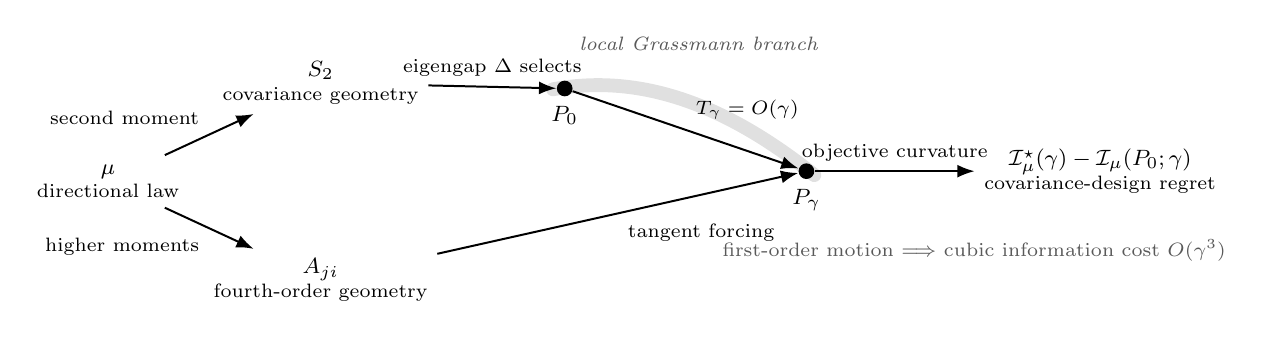
\begin{tikzpicture}[
  >=Latex,
  every node/.style={font=\footnotesize,align=center},
  flow/.style={-{Latex[length=2.2mm]},line width=0.72pt},
  manifold/.style={line width=5pt,draw=black!12,line cap=round},
  point/.style={circle,fill=black,inner sep=2pt}
]
  \node (law) at (0.55,1.50) {$\mu$\\[-1pt]\scriptsize directional law};
  \node (s2) at (3.25,2.75) {$S_2$\\[-1pt]\scriptsize covariance geometry};
  \node (a4) at (3.25,0.25) {$A_{ji}$\\[-1pt]\scriptsize fourth-order geometry};

  \draw[manifold] (6.20,2.67) .. controls (7.45,2.90) and (8.55,2.35) .. (9.52,1.58);
  \node[font=\scriptsize\itshape,text=black!65] at (8.05,3.25)
    {local Grassmann branch};
  \node[point,label={[font=\footnotesize]below=3pt:$P_0$}] (p0) at (6.35,2.68) {};
  \node[point,label={[font=\footnotesize]below=3pt:$P_\gamma$}] (pg) at (9.42,1.63) {};
  \node (info) at (13.15,1.63)
    {$\mathcal I_\mu^\star(\gamma)-\mathcal I_\mu(P_0;\gamma)$\\[-1pt]
     \scriptsize covariance-design regret};

  \draw[flow] (law) -- node[above left,font=\scriptsize] {second moment} (s2);
  \draw[flow] (law) -- node[below left,font=\scriptsize] {higher moments} (a4);
  \draw[flow] (s2) -- node[above,font=\scriptsize] {eigengap $\Delta$ selects} (p0);
  \draw[flow] (p0) -- node[above right,font=\scriptsize] {$T_\gamma=O(\gamma)$} (pg);
  \draw[flow] (a4) -- node[below right,font=\scriptsize] {tangent forcing} (pg);
  \draw[flow] (pg) -- node[above,font=\scriptsize] {objective curvature} (info);
  \node[font=\scriptsize,text=black!65] at (11.55,0.62)
    {first-order motion $\Longrightarrow$ cubic information cost $O(\gamma^3)$};
\end{tikzpicture}%
}
\caption{Mechanism behind covariance-design stability. The second directional
moment selects the zero-SNR base projector through its eigengap, while
fourth-order contractions drive the tangent displacement of the finite-SNR
optimizer. Local objective curvature converts this first-order geometric
motion into third-order covariance-design regret.}
\label{fig:stability_mechanism}
\end{figure}

\subsection{Isotropic Covariance and Higher-Order Geometry}
When
\begin{equation}
S_2=\frac1d I_d,
\label{eq:isotropic_cov}
\end{equation}
we have $M_1(P)=K/d$ for every rank-$K$ projector.

\begin{corollary}[Fourth-order selection under isotropic covariance]\label{cor:fourth}
For \eqref{eq:isotropic_cov} and any input with $h_R\in C^3([0,\gamma_0])$, $h_R'(0)=1/2$, and $h_R''(0)=-1/2$,
\begin{equation}
\I_\mu(P;\gamma)
=\frac{K}{2d}\gamma-\frac{1}{4}M_2(P;\mu)\gamma^2+O(\gamma^3)
\end{equation}
uniformly over $P$. Hence
\begin{equation}
\I_\mu^\star(\gamma)
=\frac{K}{2d}\gamma-\frac{\gamma^2}{4}\min_{P\in\Pset}M_2(P;\mu)+O(\gamma^3).
\label{eq:isotropic_selector}
\end{equation}
Every accumulation point of optimizers as $\gamma\downarrow0$ minimizes $M_2(P;\mu)$.
\end{corollary}
\begin{proof}
Since $M_1(P)=K/d$, the first-order coefficient is identical for all $P$. Lemma~\ref{lem:expansion} with $r=2$ leaves $-M_2/4$ as the first potentially orientation-dependent coefficient, proving \eqref{eq:isotropic_selector}. Uniformity gives the optimizer statement.
\end{proof}

\begin{remark}
This corollary identifies a concrete sense in which second-order directional statistics can be informationally insufficient: if $S_2$ is isotropic, fourth-degree directional geometry can select the measurement orientation. If $M_2$ is also constant, selection is deferred to a higher order; Haar isotropy never selects an orientation.
\end{remark}

\section{Sharp Information Benchmarks}
The stability result compares designs for a fixed law. The following bounds provide reference values across laws and clarify what the second moment alone can determine.

For $a,b>0$, $\operatorname{Beta}(a,b)$ is the distribution on $(0,1)$ with density $c^{a-1}(1-c)^{b-1}/B(a,b)$, where $B(a,b)=\int_0^1t^{a-1}(1-t)^{b-1}\,dt$ is the beta function. Define
\begin{equation}
\Bbase_{d,K,R}(\gamma)=\EE_C[h_R(\gamma C)],\quad
C\sim\operatorname{Beta}\!\left(\frac K2,\frac{d-K}{2}\right).
\label{eq:Bbase}
\end{equation}
Write $\sigma$ for the Haar-uniform directional law. For Gaussian amplitudes, abbreviate $\Bbase_{d,K,R}$ as $\Bbase_{d,K}$.

\begin{theorem}[Sharp information sandwich]\label{thm:sandwich}
For the centered unit-variance amplitude in the model, every directional law $\mu$ and every $\gamma\ge0$ satisfy
\begin{equation}
\Bbase_{d,K,R}(\gamma)\le\I_\mu^\star(\gamma)
\le h_R\!\left(\gamma a_K(S_2)\right).
\label{eq:sandwich}
\end{equation}
Both endpoints are sharp in the following senses.

\emph{(a) Least-favorable directional law.} For every rank-$K$ projector, $\I_\sigma(P;\gamma)=\Bbase_{d,K,R}(\gamma)$, and hence
\begin{equation}
\inf_\mu\I_\mu^\star(\gamma)=\Bbase_{d,K,R}(\gamma).
\end{equation}

\emph{(b) Prescribed second moment.} For every positive semidefinite matrix $S$ with $\tr S=1$, a finite directional law with $S_2=S$ attains
\begin{equation}
\I_\mu^\star(\gamma)=h_R(\gamma a_K(S))
\end{equation}
for every $\gamma\ge0$ and every admissible amplitude law. Here $a_K(S)$ is the sum of the $K$ largest eigenvalues of $S$.
\end{theorem}
\begin{proof}
Let $P_H$ be a rank-$K$ projector with the rotation-invariant uniform (Haar) law. For each fixed unit $u$,
\begin{equation}
u^{\top}P_Hu\sim\operatorname{Beta}\!\left(\frac K2,\frac{d-K}{2}\right).
\label{eq:beta}
\end{equation}
Averaging $\I_\mu(P_H;\gamma)$ over $P_H$ gives $\Bbase_{d,K,R}(\gamma)$, so at least one deterministic projector has value no smaller than this average. If instead $U$ is Haar-uniform and $P$ is fixed, the same projection law holds, proving (a).

Concavity and monotonicity of $h_R$, followed by Ky Fan's maximum principle, give
\begin{equation}
\I_\mu(P;\gamma)\le h_R(\gamma\tr(PS_2))
\le h_R(\gamma a_K(S_2)).
\label{eq:jensen}
\end{equation}
For (b), write $S=V\operatorname{diag}(\lambda_1,\ldots,\lambda_d)V^{\top}$, where $V$ is orthogonal and the eigenvalues are in nonincreasing order. Set
\begin{equation}
U=V(\sqrt{\lambda_1}\varepsilon_1,\ldots,\sqrt{\lambda_d}\varepsilon_d)^{\top},
\end{equation}
where the $\varepsilon_i$ are independent equiprobable signs. Then $\|U\|=1$ and $\EE UU^{\top}=S$. The leading eigenspace projector has constant coverage $a_K(S)$ and attains the upper endpoint.
\end{proof}

An isotropic second moment alone does not give equality in (a). Likewise, (b) is sharp over laws with the specified moment and need not be tight for each individual law. Subtracting \eqref{eq:sandwich} from full-observation information gives the corresponding loss bounds,
\begin{equation}
h_R(\gamma)-h_R(\gamma a_K(S_2))\le\Lloss_\mu^\star(\gamma)
\le h_R(\gamma)-\Bbase_{d,K,R}(\gamma).
\label{eq:loss_sandwich}
\end{equation}
The recoverable directional-structure gain $G_\mu(K,\gamma)=\I_\mu^\star(\gamma)-\Bbase_{d,K,R}(\gamma)$ consequently lies between zero and $h_R(\gamma a_K(S_2))-\Bbase_{d,K,R}(\gamma)$.

\subsection{Supporting Curvature Refinement}
\begin{proposition}[Uniform curvature penalty]
Suppose $h_R\in C^2([0,\gamma])$ and $-h_R''(s)\ge\kappa$ there for a constant $\kappa\ge0$. For any coverage variable $C\in[0,1]$, let $\operatorname{Var}(C)=\EE[(C-\EE C)^2]$. Then
\begin{equation}
\EE[h_R(\gamma C)]\le h_R(\gamma\EE C)
-\frac{\kappa\gamma^2}{2}\operatorname{Var}(C).
\label{eq:curvature_penalty}
\end{equation}
For Gaussian input one may take $\kappa=1/[2(1+\gamma)^2]$.
\end{proposition}
\begin{proof}
Taylor-expand around $\gamma\EE C$ and use the lower bound on $-h_R''$. The expected first-order term vanishes.
\end{proof}
This is a Jensen-gap refinement. Larger variance alone does not order two laws with the same mean. A valid ordering follows under convex order: $C_1\preceq_{\rm cx}C_2$ means $\EE\phi(C_1)\le\EE\phi(C_2)$ for every convex $\phi$, in which case concavity gives $\EE h_R(\gamma C_1)\ge\EE h_R(\gamma C_2)$.


\section{Directional-Law Stability and Finite Representation}
This section fixes the measurement class and replaces the directional law. We first
control information and transferred-design performance, then give conditions that
also control optimizer distance and a finite-sample guarantee for an unknown law.
Moment matching gives an algebraic representation guarantee ordered by powers of
SNR, whereas projective-Wasserstein distance gives a finite-SNR metric
perturbation guarantee without requiring polynomial moment matching.

\subsection{Coverage Equivalence and Even Moments}
\begin{definition}[Order-$r$ coverage equivalence]
For an integer $r\ge1$, directional laws $\mu$ and $\nu$ are order-$r$ coverage-equivalent at rank $K$ if
\begin{equation}
M_n(P;\mu)=M_n(P;\nu),\qquad n=1,\ldots,r,
\label{eq:equiv_def}
\end{equation}
for every $P\in\Pset$.
\end{definition}

Every coverage objective is unchanged by replacing $u$ with $-u$, so only the law of $uu^{\top}$ is relevant. Write $U^{\otimes 2r}$ for the $2r$-fold tensor product of $U$ and define the symmetric moment tensor
\begin{equation}
\mathsf T_{2r}(\mu)=\EE_\mu[U^{\otimes 2r}].
\end{equation}
Contracting pairs of indices recovers lower even moments because $\|U\|^2=1$. Tensor equality therefore matches all even polynomial averages of degree at most $2r$ on the sphere.

\begin{lemma}[Rank-one characterization]\label{lem:characterization}
For probability laws $\mu,\nu$ on $\mathbb S^{d-1}$, the following are equivalent:
\begin{enumerate}
\item $\mathsf T_{2r}(\mu)=\mathsf T_{2r}(\nu)$.
\item The laws are order-$r$ coverage-equivalent at rank one.
\item For Gaussian input, the supremum of $|\I_\mu(P;\gamma)-\I_\nu(P;\gamma)|$ over rank-one projectors is $O(\gamma^{r+1})$ as $\gamma\downarrow0$.
\end{enumerate}
These conditions imply order-$r$ coverage equivalence for every rank $K$.
\end{lemma}
\begin{proof}
Tensor equality matches the polynomial $C_P(u)^n$ for every rank and $n\le r$. Conversely, rank-one matching at order $r$ gives equality of $\EE[(v^{\top}U)^{2r}]$ for every unit $v$, hence every $v\in\R^d$ by homogeneity. The coefficients of this polynomial determine the symmetric tensor. Lemma~\ref{lem:expansion} makes moment matching imply the uniform information order. For the converse, each Gaussian Taylor coefficient $(-1)^{n+1}/(2n)$ is nonzero. For every fixed rank-one projector, an information difference of order $O(\gamma^{r+1})$ forces the coefficients through order $r$ to vanish.
\end{proof}

When the target law is Haar measure, matching this tensor is the even-polynomial exactness condition of a weighted real projective $r$-design \cite{hughes2021}. The general object used below is a weighted moment-preserving cubature law; it need not be a classical unweighted design. Odd-polynomial conditions of full spherical designs are unnecessary: the uniform law on $e_1,\ldots,e_d$ and its antipodal symmetrization have identical coverage moments at every order, although the former has nonzero mean. No converse from a single higher rank to tensor equality is needed here.

\subsection{Uniform Information and Design-Transfer Guarantees}
\begin{theorem}[Information-preserving directional representation]\label{thm:representation}
Let $r\ge1$, $\gamma_0>0$, and $h_R\in C^{r+1}([0,\gamma_0])$. The following hold for $0\le\gamma\le\gamma_0$.

\emph{(a) Approximation of objectives and optimal values.} Let
$\varepsilon_n\ge0$, $1\le n\le r$, be bounds on the coverage-moment
errors at a fixed rank $K$, so that
\begin{equation}
\sup_{P\in\Pset}|M_n(P;\mu)-M_n(P;\nu)|\le\varepsilon_n,
\quad 1\le n\le r,
\end{equation}
With the coefficients $b_n$ of Lemma~\ref{lem:expansion}, define
\begin{equation}
\delta(\gamma)=\sum_{n=1}^r|b_n|\gamma^n\varepsilon_n
+\frac{2\gamma^{r+1}}{(r+1)!}\sup_{0\le s\le\gamma}|h_R^{(r+1)}(s)|.
\label{eq:representation_delta}
\end{equation}
Then
\begin{align}
\sup_{P\in\Pset}|\I_\mu(P;\gamma)-\I_\nu(P;\gamma)|&\le\delta(\gamma),\label{eq:equiv_bound}\\
|\I_\mu^\star(\gamma)-\I_\nu^\star(\gamma)|&\le\delta(\gamma).\label{eq:optimal_equiv_bound}
\end{align}
In particular, exact coverage matching sets every $\varepsilon_n$ to zero and gives a uniform $O(\gamma^{r+1})$ error.

\emph{(b) Transfer of measurement designs.} If $P_\nu$ is $\eta$-optimal for the surrogate, meaning $\I_\nu^\star-\I_\nu(P_\nu;\gamma)\le\eta$ for $\eta\ge0$, then
\begin{equation}
0\le\I_\mu^\star(\gamma)-\I_\mu(P_\nu;\gamma)\le2\delta(\gamma)+\eta.
\label{eq:compression_regret}
\end{equation}
The same conclusion holds with any valid uniform objective-error bound replacing $\delta(\gamma)$.

\emph{(c) Finite directional representation.} Write $\delta_u$ for unit
point mass at $u$ and $\operatorname{supp}\mu$ for the smallest closed set
of full $\mu$-measure. For every law $\mu$, there is a weighted law
\begin{equation}
\nu_r=\sum_{\ell=1}^m w_\ell\delta_{u_\ell},\qquad
w_\ell>0,\quad\sum_{\ell=1}^m w_\ell=1,
\end{equation}
with every node $u_\ell$ in $\operatorname{supp}\mu$ and
\begin{equation}
m\le D_{d,r}\triangleq\binom{d+2r-1}{2r},\qquad
\mathsf T_{2r}(\nu_r)=\mathsf T_{2r}(\mu).
\label{eq:support_bound}
\end{equation}
Here $m$ is the number of nodes and $\binom{n}{k}=n!/[k!(n-k)!]$ is the binomial coefficient. The same $\nu_r$ satisfies (a) and (b), with zero moment errors, simultaneously for every measurement rank.
\end{theorem}
\begin{proof}
\emph{(a)} Subtract the uniform expansions in Lemma~\ref{lem:expansion}. Each coefficient difference is bounded by $|b_n|\gamma^n\varepsilon_n$, and the two remainder bounds add. The optimal-value bound follows from $|\max f-\max g|\le\sup|f-g|$.

\emph{(b)} For an original-law optimizer $P_\mu$, insert and subtract the surrogate values at $P_\mu$ and $P_\nu$ in $\I_\mu(P_\mu;\gamma)-\I_\mu(P_\nu;\gamma)$. The two approximation errors contribute at most $2\delta(\gamma)$ and surrogate suboptimality contributes at most $\eta$.

\emph{(c)} Consider the $D_{d,r}$ homogeneous monomials of degree $2r$ restricted to the sphere. They are linearly independent, since a homogeneous polynomial vanishing on the sphere vanishes everywhere by radial scaling. Multiplying a lower even-degree monomial by a power of $\sum_i u_i^2=1$ shows that they span all even polynomials through degree $2r$ on the sphere.

Let $\Phi(u)$ be the vector of these monomials. Its image on the compact set $\operatorname{supp}\mu$ lies in an affine hyperplane, because $(\sum_i u_i^2)^r=1$. The vector $\EE_\mu\Phi(U)$ lies in its convex hull. Carath\'eodory's theorem represents it by at most $D_{d,r}$ image points; discard zero weights. This is the classical finite-dimensional cubature argument underlying Tchakaloff's theorem \cite{bayer2006}. Lemma~\ref{lem:characterization} supplies exact coverage matching for every rank, and (a)--(b) give the information guarantees.
\end{proof}

\begin{corollary}[Gaussian error at every finite SNR]\label{cor:gaussian_representation}
For Gaussian amplitudes and order-$r$ coverage-equivalent laws at rank $K$, let $q=\gamma/(\gamma+2)$ and define
\begin{equation}
\delta_r(\gamma)=\min\left\{\frac{\gamma^{r+1}}{2(r+1)},
\frac{q^{r+1}}{(r+1)(1-q)}\right\}.
\label{eq:compression_delta}
\end{equation}
For every finite $\gamma\ge0$, both the uniform objective error and optimal-value error are at most $\delta_r(\gamma)$. A globally optimal surrogate design has original-law regret at most $2\delta_r(\gamma)$. The finite surrogate of Theorem~\ref{thm:representation}(c) has these guarantees at every rank. At fixed positive finite SNR, the error bound converges geometrically in $r$.
\end{corollary}
\begin{proof}
For $h_R(s)=\tfrac12\log(1+s)$, the exact signed remainder after degree $r$ is
\begin{equation}
\mathcal R_{r+1}^{\rm G}(c)=\frac{(-1)^r}{2}\int_0^{\gamma c}\frac{t^r}{1+t}\,dt.
\label{eq:signed_remainder}
\end{equation}
Its values on $0\le c\le1$ lie in an interval of length at most $\gamma^{r+1}/[2(r+1)]$. After polynomial cancellation, the difference of two expectations is bounded by this interval length.

For the complementary bound, write
\begin{equation}
\tfrac12\log(1+\gamma c)=\tfrac12\log(1+\gamma/2)
+\tfrac12\log(1+q(2c-1)).
\end{equation}
The second logarithm's degree-$r$ polynomial has uniform remainder at most $q^{r+1}/[2(r+1)(1-q)]$. Coverage matching cancels this polynomial and the two remainder bounds add. Theorem~\ref{thm:representation}(a)--(b) transfers the resulting objective bound to optimal values and design regret.
\end{proof}

For a prescribed SNR interval $0\le\gamma\le\Gamma$ with $\Gamma>0$, the same Gaussian surrogate has uniform error at most $\delta_r(\Gamma)$. For $0<\epsilon<1$, set $q_\Gamma=\Gamma/(\Gamma+2)$. It suffices to choose $r\ge1$ with
\begin{equation}
r+1\ge\frac{\log[1/(\epsilon(1-q_\Gamma))]}{-\log q_\Gamma}
\label{eq:error_budget}
\end{equation}
to obtain error at most $\epsilon$ and transfer regret at most $2\epsilon$. At fixed $d$ and $\Gamma$, the sufficient support size is $O((\log(1/\epsilon))^{d-1})$. This is a cubature-existence guarantee, not a computational-efficiency bound; the statistical sample requirement is treated below. For example, $D_{8,1}=36$, $D_{8,2}=330$, and $D_{8,3}=1716$, so the bound need not compress a smaller original law. For finite laws, linear moment constraints provide a constructive route, with residual moment errors covered by Theorem~\ref{thm:representation}(a).

\begin{proposition}[Projective-Wasserstein law perturbation]
\label{prop:wasserstein}
For $u,v\in\mathbb S^{d-1}$, define the projective distance
\begin{equation}
\rho(u,v)=\min\{\|u-v\|,\|u+v\|\}
=\sqrt{2-2|u^{\top}v|}.
\label{eq:projective_distance}
\end{equation}
For laws $\mu$ and $\nu$ on the sphere, define their projective
Wasserstein-1 distance by
\begin{equation}
W_1^{\rm proj}(\mu,\nu)=\inf_{\pi\in\Pi(\mu,\nu)}
\int\rho(u,v)\,d\pi(u,v),
\label{eq:wasserstein_definition}
\end{equation}
where $\Pi(\mu,\nu)$ is the set of couplings with marginals $\mu$ and $\nu$.
Equivalently, this is the Wasserstein-1 distance between the laws induced on
real projective space, so antipodal redistribution has zero distance.
If $h_R\in C^1([0,\gamma])$ and
$L_\gamma=\sup_{0\le s\le\gamma}|h_R'(s)|$, then
\begin{equation}
\sup_{P\in\Pset}|\I_\mu(P;\gamma)-\I_\nu(P;\gamma)|
\le \gamma L_\gamma W_1^{\rm proj}(\mu,\nu).
\label{eq:wasserstein_objective}
\end{equation}
Consequently, every $\eta$-optimal design $P_\nu$ for $\nu$ satisfies
\begin{equation}
\I_\mu^\star(\gamma)-\I_\mu(P_\nu;\gamma)
\le2\gamma L_\gamma W_1^{\rm proj}(\mu,\nu)+\eta.
\label{eq:wasserstein_regret}
\end{equation}
For Gaussian amplitudes, $L_\gamma=1/2$, so the objective error in
\eqref{eq:wasserstein_objective} is at most
$\gamma W_1^{\rm proj}(\mu,\nu)/2$.
\end{proposition}
\begin{proof}
Choose $\varepsilon\in\{-1,1\}$ so that
$\theta=\arccos(u^{\top}\varepsilon v)=\arccos|u^{\top}v|\in[0,\pi/2]$.
The two nonzero eigenvalues of
$uu^{\top}-(\varepsilon v)(\varepsilon v)^{\top}=uu^{\top}-vv^{\top}$ are
$\sin\theta$ and $-\sin\theta$. Ky Fan's inequalities therefore give, for
every $P\in\Pset$,
\begin{equation}
|u^{\top}Pu-v^{\top}Pv|
\le\sin\theta
=\rho(u,v)\cos(\theta/2)
\le\rho(u,v).
\end{equation}
Thus $u\mapsto h_R(\gamma u^{\top}Pu)$ is
$\gamma L_\gamma$-Lipschitz, uniformly in $P$. Integrating under any
coupling and then taking the infimum proves \eqref{eq:wasserstein_objective}.
Theorem~\ref{thm:representation}(b) gives \eqref{eq:wasserstein_regret}.
\end{proof}

Figure~\ref{fig:projective_quotient} shows why the shorter of the two
antipodal chords enters the perturbation bound.
\ProjectiveSphereFigure

\begin{corollary}[Optimizer stability under law replacement]
\label{cor:law_optimizer}
Let
\begin{equation}
e_\gamma=\sup_{P\in\Pset}
|\I_\mu(P;\gamma)-\I_\nu(P;\gamma)|,
\end{equation}
and let $\mathcal M_\mu(\gamma)$ be the nonempty set of maximizers of
$\I_\mu(\cdot;\gamma)$. Define
$\operatorname{dist}_F(P,\mathcal M)=\inf_{Q\in\mathcal M}\|P-Q\|_F$.
Suppose the original-law objective has quadratic growth:
for some $\kappa>0$,
\begin{equation}
\I_\mu^\star(\gamma)-\I_\mu(P;\gamma)
\ge \frac{\kappa}{2}\operatorname{dist}_F
   (P,\mathcal M_\mu(\gamma))^2,
\qquad P\in\Pset.
\label{eq:quadratic_growth_law}
\end{equation}
If $P_\nu$ is $\eta$-optimal for $\nu$, then
\begin{equation}
\operatorname{dist}_F(P_\nu,\mathcal M_\mu(\gamma))
\le \sqrt{\frac{2(2e_\gamma+\eta)}{\kappa}}.
\label{eq:law_optimizer_distance}
\end{equation}
In Theorem~\ref{thm:representation}(a), one may replace $e_\gamma$ by
$\delta(\gamma)$. If the original-law optimizer is unique, this is a direct
Frobenius-distance bound between the transferred and original optimizers.
\end{corollary}
\begin{proof}
The comparison in Theorem~\ref{thm:representation}(b), with the exact uniform
error $e_\gamma$, gives
$\I_\mu^\star-\I_\mu(P_\nu;\gamma)\le2e_\gamma+\eta$.
Combining this inequality with \eqref{eq:quadratic_growth_law} proves
\eqref{eq:law_optimizer_distance}.
\end{proof}

\begin{remark}[When quadratic growth is available]
On the Grassmann manifold, a strict isolated maximizer whose negative objective
has a positive-definite Riemannian Hessian satisfies a local quadratic-growth
condition. Extending that condition to all of $\Pset$, as assumed in
\eqref{eq:quadratic_growth_law}, additionally requires separation of the
objective from its optimum away from the maximizing set. Uniqueness alone does
not imply quadratic growth.
\end{remark}

\begin{corollary}[Joint SNR--directional-law stability]
\label{cor:joint_perturbation}
Let $\gamma,\gamma'\in[0,\Gamma]$, suppose $h_R\in C^1([0,\Gamma])$, and set
\begin{equation}
L_\Gamma=\sup_{0\le s\le\Gamma}|h_R'(s)|,
\qquad
\epsilon_{\gamma,\gamma'}
=L_\Gamma|\gamma-\gamma'|
+L_\Gamma\min\{\gamma,\gamma'\}W_1^{\rm proj}(\mu,\nu).
\label{eq:joint_error}
\end{equation}
Then
\begin{equation}
\sup_{P\in\Pset}|\I_\mu(P;\gamma)-\I_\nu(P;\gamma')|
\le\epsilon_{\gamma,\gamma'}.
\label{eq:joint_objective}
\end{equation}
If $P_{\nu,\gamma'}$ is $\eta$-optimal for law $\nu$ at SNR $\gamma'$, then
\begin{equation}
\I_\mu^\star(\gamma)-\I_\mu(P_{\nu,\gamma'};\gamma)
\le2\epsilon_{\gamma,\gamma'}+\eta.
\label{eq:joint_regret}
\end{equation}
If the target objective $\I_\mu(\cdot;\gamma)$ satisfies
\eqref{eq:quadratic_growth_law} with constant $\kappa$, then
\begin{equation}
\operatorname{dist}_F(P_{\nu,\gamma'},\mathcal M_\mu(\gamma))
\le\sqrt{\frac{2(2\epsilon_{\gamma,\gamma'}+\eta)}{\kappa}}.
\label{eq:joint_optimizer}
\end{equation}
\end{corollary}
\begin{proof}
For every $c\in[0,1]$,
$|h_R(\gamma c)-h_R(\gamma'c)|\le L_\Gamma|\gamma-\gamma'|$.
If $\gamma\le\gamma'$, insert $\I_\nu(P;\gamma)$ between the two objectives;
if $\gamma'\le\gamma$, insert $\I_\mu(P;\gamma')$ instead.
Proposition~\ref{prop:wasserstein} then gives the projective-Wasserstein term at the
smaller SNR, proving \eqref{eq:joint_objective}. The comparison argument of
Theorem~\ref{thm:representation}(b) proves \eqref{eq:joint_regret}, and
Corollary~\ref{cor:law_optimizer} proves \eqref{eq:joint_optimizer}.
\end{proof}

For Gaussian amplitudes, $L_\Gamma=1/2$, so the joint error specializes to
\begin{equation}
\epsilon_{\gamma,\gamma'}
= \frac12|\gamma-\gamma'|
+\frac12\min\{\gamma,\gamma'\}W_1^{\rm proj}(\mu,\nu).
\label{eq:joint_gaussian}
\end{equation}

The next result closes the gap between a known directional law and one
learned from independent direction samples. Its guarantee is uniform over
the continuous projector class, rather than over a finite numerical
candidate set.

\begin{corollary}[Finite-sample learned-law guarantee]
\label{cor:finite_sample}
Let $N,r\ge1$, let $U_1,\ldots,U_N$ be independent samples from $\mu$, let $\gamma>0$, and
suppose $h_R\in C^{r+1}([0,\gamma])$. Define the empirical law
$\widehat\mu_N=N^{-1}\sum_{i=1}^N\delta_{U_i}$ and set
\begin{equation}
L_\gamma=\sup_{0\le s\le\gamma}|h_R'(s)|,
\qquad
H_\gamma=\sup_{0\le s\le\gamma}h_R(s)
-\inf_{0\le s\le\gamma}h_R(s),
\end{equation}
and $p_d=d(d+1)/2$. For $0<\xi\le\sqrt K$ and $0<\alpha<1$, set
\begin{equation}
\Delta_N(\xi,\alpha)=2\gamma L_\gamma\xi
+H_\gamma\sqrt{\frac{p_d\log(1+2\sqrt K/\xi)+\log(2/\alpha)}{2N}}.
\label{eq:empirical_uniform_bound}
\end{equation}
Then, with probability at least $1-\alpha$,
\begin{equation}
\sup_{P\in\Pset}|\I_\mu(P;\gamma)
-\I_{\widehat\mu_N}(P;\gamma)|
\le\Delta_N(\xi,\alpha).
\label{eq:empirical_uniform_information}
\end{equation}
Moreover, there is a weighted law $\nu_{N,r}$ supported on at most
\begin{equation}
\min\left\{N,D_{d,r}\right\}
\end{equation}
observed directions and matching the empirical even moments through degree
$2r$. With
\begin{equation}
\tau_r(\gamma)=\frac{2\gamma^{r+1}}{(r+1)!}
\sup_{0\le s\le\gamma}|h_R^{(r+1)}(s)|,
\end{equation}
the same event satisfies the following bounds for every $\eta$-optimal design
$P_{N,r}$ under $\nu_{N,r}$:
\begin{align}
\sup_{P\in\Pset}|\I_\mu(P;\gamma)-\I_{\nu_{N,r}}(P;\gamma)|
&\le \Delta_N(\xi,\alpha)+\tau_r(\gamma),
\label{eq:sample_compressed_error}\\
\I_\mu^\star(\gamma)-\I_\mu(P_{N,r};\gamma)
&\le2[\Delta_N(\xi,\alpha)+\tau_r(\gamma)]+\eta,
\label{eq:sample_compressed_regret}
\end{align}
For Gaussian amplitudes, $\tau_r(\gamma)$ may be replaced by the sharper
$\delta_r(\gamma)$ in \eqref{eq:compression_delta}. If
\eqref{eq:quadratic_growth_law} holds, the right side of
\eqref{eq:law_optimizer_distance} applies with
$e_\gamma=\Delta_N(\xi,\alpha)+\tau_r(\gamma)$.
\end{corollary}
\begin{proof}
For fixed $u$, the map $P\mapsto h_R(\gamma u^{\top}Pu)$ is
$\gamma L_\gamma$-Lipschitz in Frobenius norm. The rank-$K$ projectors lie in
the radius-$\sqrt K$ ball centered at the origin in the $p_d$-dimensional space of real symmetric
matrices. A maximal $\xi$-separated subset is a $\xi$-net with cardinality at
most $(1+2\sqrt K/\xi)^{p_d}$, by the standard disjoint-ball volume argument.
For every net point, Hoeffding's inequality \cite{hoeffding1963} bounds the
deviation of the empirical average of a variable with range $H_\gamma$.
A union bound over the net gives the square-root term in
\eqref{eq:empirical_uniform_bound}; moving from a projector to its net point
in both the population and empirical objectives adds $2\gamma L_\gamma\xi$.
This proves \eqref{eq:empirical_uniform_information}.

Apply Theorem~\ref{thm:representation}(c) to the finite law
$\widehat\mu_N$. Its nodes can be selected from the observed directions, so
the support contains at most $\min\{N,D_{d,r}\}$ points. Theorem
\ref{thm:representation}(a) bounds the empirical-to-compressed error by
$\tau_r(\gamma)$. The triangle inequality gives
\eqref{eq:sample_compressed_error}, and Theorem~\ref{thm:representation}(b)
gives \eqref{eq:sample_compressed_regret}. The Gaussian and optimizer-distance
claims follow from Corollaries~\ref{cor:gaussian_representation} and
\ref{cor:law_optimizer}, respectively.
\end{proof}

For an explicit accuracy statement, let $L_\gamma>0$, choose a target
$\zeta>0$, and set
$\xi_\zeta=\min\{\sqrt K,\zeta/(4\gamma L_\gamma)\}$. The sufficient condition
\begin{equation}
N\ge \frac{2H_\gamma^2}{\zeta^2}
\left[p_d\log\!\left(1+\frac{2\sqrt K}{\xi_\zeta}\right)
+\log\!\left(\frac2\alpha\right)\right]
\label{eq:sample_complexity}
\end{equation}
gives $\Delta_N(\xi_\zeta,\alpha)\le\zeta$. Thus, apart from the displayed
dimension and logarithmic factors, the directional sample size scales as
$\zeta^{-2}$.

\begin{remark}[Ambient versus intrinsic covering dimension]
The covering argument in \eqref{eq:empirical_uniform_bound} deliberately
embeds $\Pset$ in the $p_d=d(d+1)/2$ dimensional space of symmetric matrices,
which gives an explicit self-contained bound. Direct metric-entropy bounds for
the rank-$K$ Grassmann manifold can replace this ambient exponent by one that
scales with its intrinsic dimension $K(d-K)$, at the cost of additional
covering constants \cite{dai2008}. We retain the ambient argument so the stated
finite-sample constant follows from the elementary volume bound alone.
\end{remark}

\subsection{Spherical Designs and Explicit Ensembles}
A spherical $t$-design reproduces spherical averages of all polynomials of degree at most $t$ \cite{delsarte1977}. It is therefore sufficient, though not necessary, for even-moment matching.
\begin{corollary}[Spherical-design information preservation]\label{cor:design}
Let $\mu_r$ be a spherical $2r$-design and $\sigma$ the Haar law. Under the regularity assumption of Theorem~\ref{thm:representation},
\begin{equation}
\sup_{P\in\Pset}|\I_{\mu_r}(P;\gamma)-\I_\sigma(P;\gamma)|
\le\frac{2\gamma^{r+1}}{(r+1)!}\sup_{0\le s\le\gamma}|h_R^{(r+1)}(s)|.
\label{eq:design_bound}
\end{equation}
For Gaussian input, the sharper bound $\delta_r(\gamma)$ holds.
\end{corollary}
\begin{proof}
Each $C_P(u)^n$ is a polynomial of degree $2n$. A spherical $2r$-design therefore matches coverage moments for $n\le r$. Apply Theorem~\ref{thm:representation}(a) and Corollary~\ref{cor:gaussian_representation}.
\end{proof}


Figure~\ref{fig:law_stability_mechanism} shows how the algebraic, transport,
and finite-data routes feed the same uniform information error before that
error is propagated to design-level guarantees.
\begin{figure}[H]
\centering
\resizebox{0.96\textwidth}{!}{%
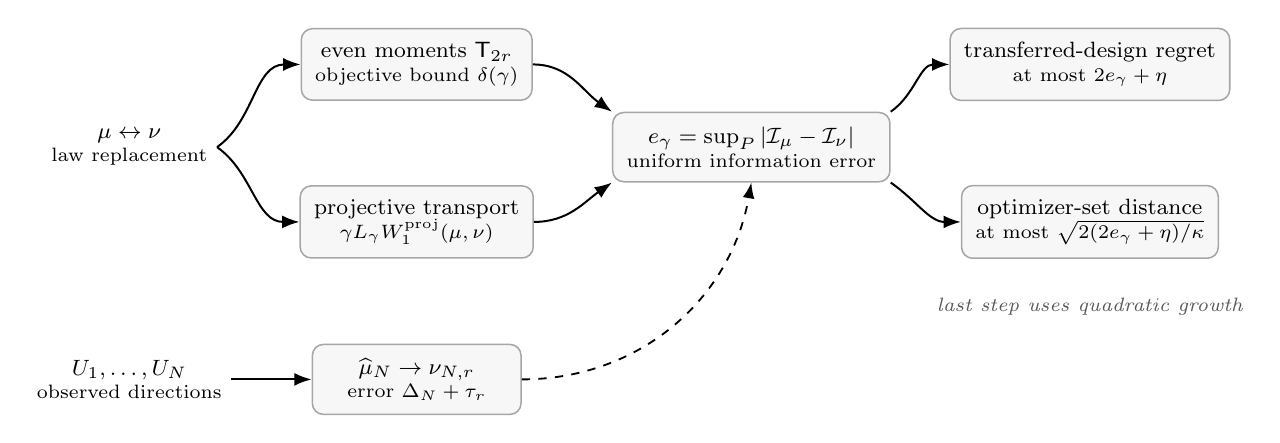
\begin{tikzpicture}[
  >=Latex,
  every node/.style={font=\footnotesize,align=center},
  flow/.style={-{Latex[length=2.2mm]},line width=0.72pt},
  dataflow/.style={-{Latex[length=2mm]},line width=0.66pt,dashed},
  stage/.style={draw=black!35,fill=black!3,line width=0.55pt,
                rounded corners=4pt,minimum width=2.65cm,minimum height=0.88cm,
                inner sep=5pt}
]
  \node (laws) at (0.15,2.40) {$\mu\leftrightarrow\nu$\\[-1pt]
    \scriptsize law replacement};
  \node[stage] (mom) at (3.80,3.45)
    {even moments $\mathsf T_{2r}$\\[-1pt]
     \scriptsize objective bound $\delta(\gamma)$};
  \node[stage] (wass) at (3.80,1.45)
    {projective transport\\[-1pt]
     \scriptsize $\gamma L_\gamma W_1^{\rm proj}(\mu,\nu)$};
  \node[stage,minimum width=3.15cm] (err) at (8.05,2.40)
    {$e_\gamma=\sup_P|\mathcal I_\mu-\mathcal I_\nu|$\\[-1pt]
     \scriptsize uniform information error};
  \node[stage] (reg) at (12.35,3.45)
    {transferred-design regret\\[-1pt]
     \scriptsize at most $2e_\gamma+\eta$};
  \node[stage] (geo) at (12.35,1.45)
    {optimizer-set distance\\[-1pt]
     \scriptsize at most $\sqrt{2(2e_\gamma+\eta)/\kappa}$};
  \node (data) at (0.15,-0.55)
    {$U_1,\ldots,U_N$\\[-1pt]\scriptsize observed directions};
  \node[stage] (emp) at (3.80,-0.55)
    {$\widehat\mu_N\rightarrow\nu_{N,r}$\\[-1pt]
     \scriptsize error $\Delta_N+\tau_r$};

  \draw[flow] (laws.east) to[out=35,in=180] (mom.west);
  \draw[flow] (laws.east) to[out=-35,in=180] (wass.west);
  \draw[flow] (mom.east) to[out=0,in=145] (err.north west);
  \draw[flow] (wass.east) to[out=0,in=215] (err.south west);
  \draw[flow] (err.north east) to[out=35,in=180] (reg.west);
  \draw[flow] (err.south east) to[out=-35,in=180] (geo.west);
  \draw[flow] (data.east) -- (emp.west);
  \draw[dataflow] (emp.east) to[out=0,in=260] (err.south);

  \node[font=\scriptsize\itshape,text=black!65] at (12.35,0.38)
    {last step uses quadratic growth};
\end{tikzpicture}%
}
\caption{Two routes from directional-law mismatch to operational guarantees.
Even-moment control and projective transport bound the same uniform information
discrepancy. A comparison argument propagates it to transferred-design regret;
quadratic growth further converts it into optimizer-set distance. The empirical
and cubature path supplies the finite-data realization of the moment route.}
\label{fig:law_stability_mechanism}
\end{figure}

\subsubsection{Canonical finite ensembles}
The numerical study considers three finite ensembles in $d=3$. The antipodal coordinate axes provide a low-order discrete benchmark with isotropic second moment. The regular tetrahedron provides a compact noncontinuous spherical design. The regular icosahedron is a tight spherical 5-design in three dimensions \cite{reznick1995}. Their role is not to introduce new designs, but to test the predicted information-preservation order.

\begin{proposition}[Explicit second- and third-order separation]\label{prop:examples}
Let $d=3$, $K=1$, and let the amplitude be Gaussian. For uniform antipodal coordinate axes and for the regular tetrahedron,
\begin{equation}
\I_\mu^\star(\gamma)=\tfrac12\log(1+\gamma/3),\qquad
\I_\mu^\star(\gamma)-\Bbase_{3,1}(\gamma)=\frac{\gamma^2}{45}+O(\gamma^3).
\end{equation}
For the uniform regular icosahedron, let $\I_{\rm vertex}(\gamma)$ denote the
information achieved by projecting onto any vertex. Then
\begin{equation}
\begin{split}
\I_{\rm vertex}(\gamma)&=\frac1{12}\log(1+\gamma)+\frac5{12}\log(1+\gamma/5),\\
\I_{\rm vertex}(\gamma)-\Bbase_{3,1}(\gamma)&=\frac{8}{1575}\gamma^3+O(\gamma^4),
\end{split}
\label{eq:ico_witness}
\end{equation}
In particular, the optimal icosahedral gain is $\Theta(\gamma^3)$ as $\gamma\downarrow0$.
\end{proposition}
\begin{proof}
Both ensembles have $S_2=I_3/3$. For the axes, choose the measuring direction
\begin{equation*}
(1,1,1)/\sqrt3.
\end{equation*}
For tetrahedral vertices $(1,1,1)$, $(1,-1,-1)$, $(-1,1,-1)$, and $(-1,-1,1)$, normalized by $\sqrt3$, choose $e_1$. Both displayed choices give constant coverage $1/3$, and their information equals the common Jensen upper bound $h_R(\gamma/3)$. Their coverage moment $M_2$ is $1/9$, whereas Haar coverage has second moment $1/5$, giving $(1/5-1/9)/4=1/45$.
For the icosahedron, coverage along a vertex is $1$ with probability $1/6$ and $1/5$ with probability $5/6$. Its first two moments are $1/3$ and $1/5$, and its third moment is $13/75$, compared with the Haar value $1/7$. Thus the cubic coefficient is $(13/75-1/7)/6=8/1575$. This feasible projector lower-bounds the optimal gain; the spherical-design bound with $r=2$ gives the matching $O(\gamma^3)$ upper bound. No finite-SNR optimality claim is needed for the vertex projector.
\end{proof}

Figure~\ref{fig:three_dimensional_landscapes} displays the full rank-one
information landscapes behind Proposition~\ref{prop:examples}. For a unit
measurement direction
$v=(\sin\theta\cos\phi,\sin\theta\sin\phi,\cos\theta)^\top$,
write $P_v=vv^\top$. At Gaussian SNR $\gamma=3$, a uniform ensemble of
$m$ directions $u_j$ has the exact information value
\begin{equation}
\I_\mu(P_v;3)=\frac{1}{2m}\sum_{j=1}^{m}
\log\!\left(1+3(v^\top u_j)^2\right).
\label{eq:three_dimensional_surface}
\end{equation}
Each plotted mesh vertex evaluates this value in nats directly; no angular
optimization is used to generate the surface. Since $v$ and $-v$
define the same projector, the northern hemisphere $0\le\theta\le90^\circ$
contains every distinct rank-one projector, up to its boundary identification.
\pgfmathdeclarefunction{axisinfo}{2}{%
  \pgfmathparse{(ln(1+3*(sin(#1)*cos(#2))^2)
    +ln(1+3*(sin(#1)*sin(#2))^2)+ln(1+3*cos(#1)^2))/6}%
}
\pgfmathdeclarefunction{tetinfo}{2}{%
  \pgfmathparse{(
    ln(1+(sin(#1)*cos(#2)+sin(#1)*sin(#2)+cos(#1))^2)
   +ln(1+(sin(#1)*cos(#2)-sin(#1)*sin(#2)-cos(#1))^2)
   +ln(1+(-sin(#1)*cos(#2)+sin(#1)*sin(#2)-cos(#1))^2)
   +ln(1+(-sin(#1)*cos(#2)-sin(#1)*sin(#2)+cos(#1))^2))/8}%
}
\begin{figure}[H]
\centering
\begin{minipage}{0.49\textwidth}\centering
\begin{tikzpicture}
\begin{axis}[
  width=0.94\linewidth,height=6.4cm,view={55}{25},
  xlabel={$\theta$},ylabel={$\phi$},zlabel={$\mathcal I$},
  xtick={0,45,90},ytick={0,180,360},
  zmin=0.22,zmax=0.36,ztick={0.24,0.30,0.36},
  xmin=0,xmax=90,ymin=0,ymax=360,
  xlabel style={font=\scriptsize},ylabel style={font=\scriptsize},
  zlabel style={font=\scriptsize},tick label style={font=\scriptsize},
  grid=major,grid style={black!12},
  colormap={papergray}{gray(0cm)=(0.92); gray(1cm)=(0.28)},
  point meta min=0.22,point meta max=0.36,
  title={(a) Coordinate axes},title style={font=\footnotesize},
]
\addplot3[surf,shader=interp,draw=black!25,opacity=0.94,
  samples=19,samples y=25,domain=0:90,y domain=0:360]
  {axisinfo(x,y)};
\addplot3[only marks,mark=*,mark size=1.6pt,black]
  coordinates {(54.7356,45,0.3465736)};
\end{axis}
\end{tikzpicture}
\end{minipage}%
\begin{minipage}{0.49\textwidth}\centering
\begin{tikzpicture}
\begin{axis}[
  width=0.94\linewidth,height=6.4cm,view={55}{25},
  xlabel={$\theta$},ylabel={$\phi$},zlabel={$\mathcal I$},
  xtick={0,45,90},ytick={0,180,360},
  zmin=0.22,zmax=0.36,ztick={0.24,0.30,0.36},
  xmin=0,xmax=90,ymin=0,ymax=360,
  xlabel style={font=\scriptsize},ylabel style={font=\scriptsize},
  zlabel style={font=\scriptsize},tick label style={font=\scriptsize},
  grid=major,grid style={black!12},
  colormap={papergray}{gray(0cm)=(0.92); gray(1cm)=(0.28)},
  point meta min=0.22,point meta max=0.36,
  title={(b) Tetrahedron},title style={font=\footnotesize},
]
\addplot3[surf,shader=interp,draw=black!25,opacity=0.94,
  samples=19,samples y=25,domain=0:90,y domain=0:360]
  {tetinfo(x,y)};
\addplot3[only marks,mark=*,mark size=1.6pt,black]
  coordinates {(90,0,0.3465736)};
\end{axis}
\end{tikzpicture}
\end{minipage}
\caption{Exact three-dimensional information landscapes for rank-one
measurements in $d=3$ at Gaussian SNR $\gamma=3$. The horizontal coordinates
are polar and azimuthal angles in degrees; height is information in nats.
Black dots mark distinct optimal orientations with the common Jensen value
$\tfrac12\log 2$. Mesh vertices evaluate
\eqref{eq:three_dimensional_surface} directly.}
\label{fig:three_dimensional_landscapes}
\end{figure}

\section{Exact Gaussian Reference Laws}

\subsection{Real Haar Law}
For Gaussian $R$, the universal benchmark has the exact beta integral
\begin{equation}
\Bbase_{d,K}(\gamma)
=\frac12\int_0^1
\log(1+\gamma c)
\frac{c^{K/2-1}(1-c)^{(d-K)/2-1}}
{B(K/2,(d-K)/2)}\,dc.
\label{eq:beta_integral}
\end{equation}

The first two beta moments are
\begin{equation}
\EE[C]=\frac Kd,
\qquad
\EE[C^2]=\frac{K(K+2)}{d(d+2)},
\end{equation}
so
\begin{equation}
\Bbase_{d,K}(\gamma)
=\frac{K}{2d}\gamma
-\frac{K(K+2)}{4d(d+2)}\gamma^2
+O(\gamma^3).
\label{eq:haar_low}
\end{equation}

The general moment formula is $\EE C^n=(K/2)_n/(d/2)_n$, where $(a)_n=\prod_{j=0}^{n-1}(a+j)$ is the rising factorial. For $d=3,K=1$, a useful closed form is
\begin{equation}
\Bbase_{3,1}(\gamma)=\tfrac12\log(1+\gamma)-1+\frac{\arctan\sqrt\gamma}{\sqrt\gamma},\quad\gamma>0,
\end{equation}
with value zero at $\gamma=0$. At high SNR, let $\psi(x)=\frac{d}{dx}\log\Gamma(x)$ be the digamma function, where $\Gamma(x)=\int_0^\infty t^{x-1}e^{-t}\,dt$ is the gamma function for $x>0$. Then
\begin{equation}
\EE[\log C]
=\psi\!\left(\frac K2\right)-\psi\!\left(\frac d2\right),
\end{equation}
and hence
\begin{equation}
\Bbase_{d,K}(\gamma)
=\frac12\log\gamma
+\frac12\left[\psi\!\left(\frac K2\right)-\psi\!\left(\frac d2\right)\right]
+o(1).
\label{eq:haar_high}
\end{equation}
The additive high-SNR information penalty relative to full observation is therefore
\begin{equation}
\Lloss_{\rm Haar}(\gamma)\to
\frac12\left[\psi\!\left(\frac d2\right)-\psi\!\left(\frac K2\right)\right].
\label{eq:digamma}
\end{equation}
Here $\Lloss_{\rm Haar}=\tfrac12\log(1+\gamma)-\Bbase_{d,K}(\gamma)$ is the full-observation information loss under Haar directions. To justify the limit, write the difference from $\tfrac12\log\gamma$ as $\tfrac12\EE\log(C+1/\gamma)$. For $\gamma\ge1$, the absolute value is bounded by $|\log C|+\log2$, which is integrable under the Beta law. Dominated convergence applies.

\section{Reproducible Numerical Validation}
The main experiments use finite directional laws, so expectations are evaluated directly as weighted sums without Monte Carlo error. Randomized linear-program objectives use independent streams from seed $20260919$; auxiliary checks use seed $20260918$. Information is in nats. Numerical angular searches are convergence checks, not certified global optimization.

\subsection{Nonzero Subspace Displacement and Cubic Regret}
Set $d=2$, $K=1$, and let $u_j=(\cos\alpha_j,\sin\alpha_j)$ occur with probability $p_j$, with
\begin{equation}
\begin{aligned}
(\alpha_1,\ldots,\alpha_4)&=(0,0.6,1.3,2.2),\\
(p_1,\ldots,p_4)&=(0.45,0.25,0.20,0.10).
\end{aligned}
\end{equation}
Angles are in radians. Write $P_\theta=v_\theta v_\theta^{\top}$ for the projector onto $v_\theta=(\cos\theta,\sin\theta)^{\top}$, and let $\theta_\gamma$ be a maximizing measurement angle. The leading eigenvector of $S_2$ has angle $\theta_0=\CoreAngle$, eigengap $\Delta=\CoreGap$, and contraction $A=\EE[x^3y]=\CoreA$, where $x=\cos(\alpha-\theta_0)$ and $y=\sin(\alpha-\theta_0)$. For Gaussian input, \eqref{eq:tilt} predicts $(\theta_\gamma-\theta_0)/\gamma\to-A/\Delta=\CoreTilt$. Consequently,
\begin{align}
\frac{\|P_\gamma-P_0\|_F}{\gamma}&\longrightarrow\CoreDistanceLimit,\\
\frac{\I_\mu^\star(\gamma)-\I_\mu(P_0;\gamma)}{\gamma^3}
&\longrightarrow\frac{A^2}{2\Delta}=\CoreRegretLimit.
\end{align}
We evaluate $21$ logarithmically spaced SNRs from $10^{-4}$ to $1$. Stationary angles are located by derivative sign changes on $8192$ angular intervals and refined by Brent's method; the best resulting value is selected. Doubling the angular resolution changes the selected information by less than $3\times10^{-17}$ nats. Regret is evaluated with a logarithmic ratio to reduce cancellation. On $10^{-4}\le\gamma\le10^{-2}$, fitted slopes are $\CoreDistanceSlope$ for distance and $\CoreRegretSlope$ for regret. Figure~\ref{fig:stability} compares these values with the analytic leading terms and finite-SNR bounds. The nonzero coefficient demonstrates that cubic regret cannot generally be replaced by a higher-order bound.
\begin{figure}[t]
\centering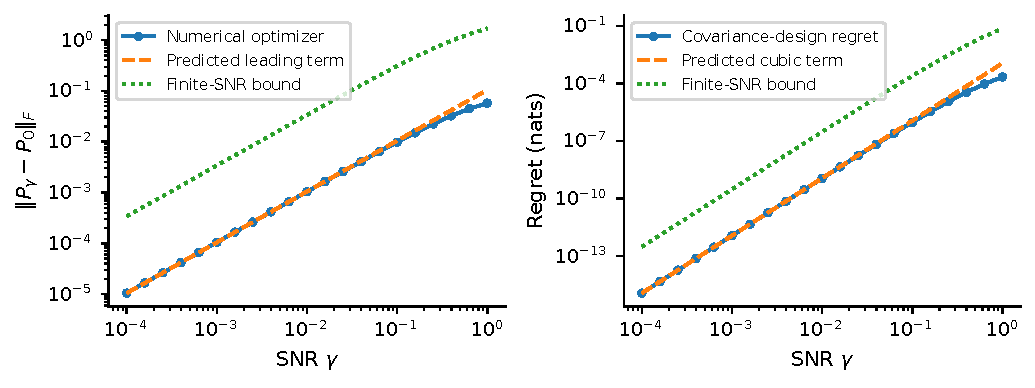
\includegraphics[width=0.95\textwidth]{figures/fig_optimizer_stability.pdf}
\caption{Gaussian four-direction example: numerical optimizer displacement (left) and covariance-design regret (right). Dashed curves use the derived leading coefficients; dotted curves are the explicit finite-SNR bounds.}
\label{fig:stability}
\end{figure}

To expose the geometry behind this displacement, embed the same four
directions as $u_j=(\cos\alpha_j,\sin\alpha_j,0)^\top\in\R^3$. Define
$b_0=(\cos\theta_0,\sin\theta_0,0)^\top$,
$b_1=(-\sin\theta_0,\cos\theta_0,0)^\top$, and $e_3=(0,0,1)^\top$.
The local unit-vector chart and its rank-one projector are
$v(t,s)=(b_0+t b_1+s e_3)/\sqrt{1+t^2+s^2}$ and
$P_{v(t,s)}=v(t,s)v(t,s)^\top$. At $\gamma=3$, denote by $P_3$ the
numerically selected information optimizer. Figure~\ref{fig:optimizer_chart_3d}
plots the information relative to the covariance projector $P_0$.
Any nonzero out-of-plane component $s$ reduces every coverage after
normalization, so an optimizer lies in the original plane; the visible
in-plane shift is the effect quantified by Corollary~\ref{cor:cubic_regret}.
\OptimizerChartFigure

\subsection{Equal Second Moments, Different Optimal Orientations}
Let $\mu_\phi$ assign equal mass to angles $\phi$ and $\phi+\pi/2$. For every $\phi$, $S_2=I_2/2$, whereas
\begin{equation}
M_2(P_\theta;\mu_\phi)=\frac38+\frac18\cos(4(\theta-\phi)).
\end{equation}
For Gaussian input and any positive SNR, the Jensen bound is attained exactly at $\theta=\phi+\pi/4$ modulo $\pi/2$, where both coverages equal $1/2$. Thus $\mu_0$ and $\mu_{\pi/6}$ have identical second moments and disjoint sets of optimal rank-one projectors. Figure~\ref{fig:orientation} shows their fourth-degree geometry and information at $\gamma=1$. This distinction is analytic; the plotted angular grid only displays it.
\begin{figure}[t]
\centering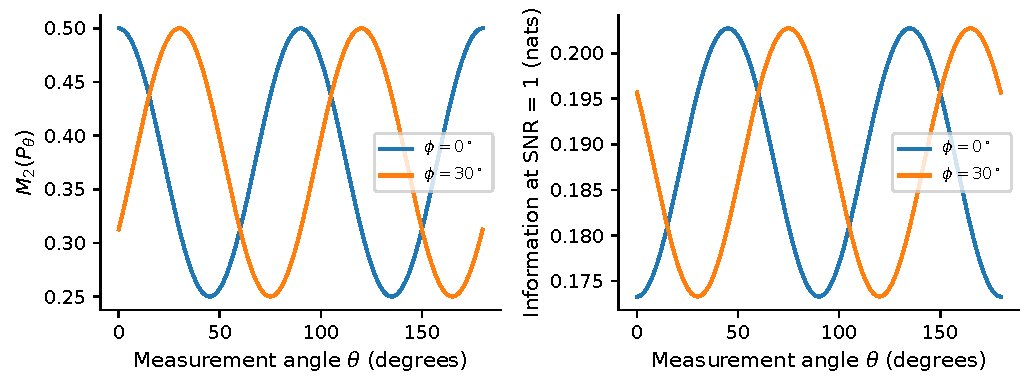
\includegraphics[width=0.95\textwidth]{figures/fig_orientation.pdf}
\caption{Two rotated directional laws with $S_2=I_2/2$. Minima of the fourth-degree coverage moment coincide with the exact information-maximizing orientations, which differ between the laws.}
\label{fig:orientation}
\end{figure}

\subsection{Compression of a Nonuniform Directional Law}
We take $41$ directions at $\alpha_j=\pi j/41$, $0\le j\le40$, with probabilities proportional to
\begin{equation}
\exp\{0.7\cos(2\alpha_j)+0.8\sin(4\alpha_j)+0.3\cos(6\alpha_j)\}.
\end{equation}
For $r\in\{1,2,3,4,6,8\}$, a linear program preserves the expectations of $1$, $\cos(2n\alpha)$, and $\sin(2n\alpha)$ for $1\le n\le r$. These functions span the even polynomial restrictions of degree at most $2r$ on the circle. A basic solution uses at most $2r+1=D_{2,r}$ directions. After least-squares refinement on the selected support, all weights remain positive; the maximum constraint residual is $\CoreMomentResidual$.

At SNRs $0.1$, $1$, and $10$, we compare original and surrogate information on $4096$ equally spaced measurement angles and transfer the numerically selected surrogate optimizer to the original law. The grid maximum is a sampled error, not the continuous supremum. At $r=4$ and $\gamma=1$, compression from $41$ to $9$ directions gives sampled information error $\CoreCompressionError$ and achieved transfer regret $\CoreCompressionRegret$ nats. The exact-matching theorem gives the respective reference bounds $1/810$ and $1/405$ nats. Figure~\ref{fig:compression} compares observed errors with these conservative guarantees. Different orders use independently chosen feasible supports, so monotonic observed error is not required.

Floating-point moment constraints are not asserted to hold exactly. The data also record a residual-aware Taylor bound from Theorem~\ref{thm:representation}(a)--(b); each coverage-moment error is at most the maximum Fourier constraint residual because the absolute Fourier coefficients of $\cos^{2n}(\theta-\alpha)$ sum to one. The plotted exact-matching bounds describe the ideal moment constraints. This deterministic compression experiment starts from a known finite law; the independent-sample guarantee is supplied separately by Corollary~\ref{cor:finite_sample}.
\begin{figure}[t]
\centering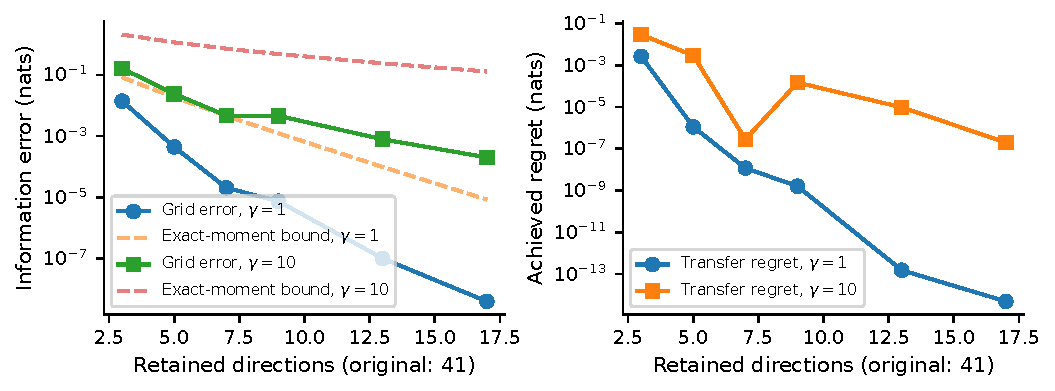
\includegraphics[width=0.95\textwidth]{figures/fig_surrogate.pdf}
\caption{Compression of a nonuniform 41-direction law. Left: sampled information errors and theoretical bounds for exact moment matching. Right: achieved transfer regret from numerical angular searches. Values below $10^{-16}$ are displayed at that floor.}
\label{fig:compression}
\end{figure}

\subsection{Finite-Sample Scaling Check}
For the same $41$-direction law and Gaussian SNR $\gamma=1$, we draw empirical
laws of sizes $N=100,400,1600$, and $6400$. Over $200$ independent repetitions,
we compute the maximum population-to-empirical information difference on the
same $4096$-angle grid. The median errors are, respectively,
$\CoreEmpiricalErrorA$, $\CoreEmpiricalErrorB$, $\CoreEmpiricalErrorC$, and
$\CoreEmpiricalErrorD$ nats. Their fitted log--log slope is
$\CoreEmpiricalSlope$, consistent with the $N^{-1/2}$ dependence in
Corollary~\ref{cor:finite_sample}. This is an empirical scaling check on a
finite angular grid, rather than a verification of the corollary's uniform
high-probability constant. The complete trial values are retained for
independent reanalysis.

\subsection{Rank-Two Design Transfer in Eight Dimensions}
To test compression beyond rank one, we fix $d=8$ and $K=2$. Define
\begin{equation}
\Sigma=\operatorname{diag}(8,5,3,2,1,1,1,1).
\end{equation}
Generate $600$ independent vectors $X_j\sim\mathcal N(0,\Sigma)$ and set $u_j=X_j/\|X_j\|$, with $u_{ji}$ denoting coordinate $i$ of direction $u_j$. The finite law assigns weights proportional to $\exp(0.6u_{j1}+0.4u_{j2}u_{j3})$. This realized finite law, not the underlying continuous Gaussian construction, is the target of compression. Reproduction uses seed $20260920$ with separate streams for directions, linear-program objectives, candidate projectors, and moment checks.

For matching orders $r=1,2$, positive linear programs preserve every homogeneous monomial of degree $2r$, together with total mass. Denote the resulting order-$r$ compressed law by $\nu_r$. Refined solutions retain $36$ and $330$ directions, respectively. At $r=3$, the support bound $D_{8,3}=1716$ exceeds the original $600$ directions, so we retain the original law as a reference rather than claim further compression. Checks on $128$ fresh projectors for each of ranks $2$ and $4$ give maximum coverage-moment residual $\RankResidual$. Thus the same surrogate weights are tested at more than one rank.

For each $\gamma\in\{1,10\}$, define a common finite candidate family $\mathcal Q_\gamma\subset\Pset$. It contains $512$ Haar projectors, the leading covariance projector, and $12$ projectors refined by projected-gradient ascent with orthonormalization. The refinements use four common starts for each of the original law and the two compressed laws. The resulting $\RankCandidates$ candidates are shared by all matching orders. Let $\widehat P_r$ maximize surrogate information over $\mathcal Q_\gamma$. Define the candidate-family information error $E_r^{\mathcal Q}$ and transfer regret $R_r^{\mathcal Q}$ by
\begin{align}
E_r^{\mathcal Q}&=\max_{P\in\mathcal Q_\gamma}|\I_\mu(P;\gamma)-\I_{\nu_r}(P;\gamma)|,\\
R_r^{\mathcal Q}&=\max_{P\in\mathcal Q_\gamma}\I_\mu(P;\gamma)-\I_\mu(\widehat P_r;\gamma).
\end{align}
These are the maximum error and transfer regret within the finite family. Exhaustive evaluation verifies $R_r^{\mathcal Q}\le2E_r^{\mathcal Q}$. The same comparison underlying Theorem~\ref{thm:representation}(a)--(b) applies to this restricted family, but these numerical values are not continuous-projector suprema or certified global-optimum regrets.

At $r=2$ and $\gamma=10$, the candidate information error is $\RankError$ nats and transfer regret is $\RankRegret$ nats. Figure~\ref{fig:rank_transfer} reports both quantities versus matching order. The third-order reference reproduces the original objective up to rounding because it uses the original law. This example directly tests measurement transfer for $K>1$ and also illustrates why an existence bound need not provide useful compression at every dimension and order.
\begin{figure}[t]
\centering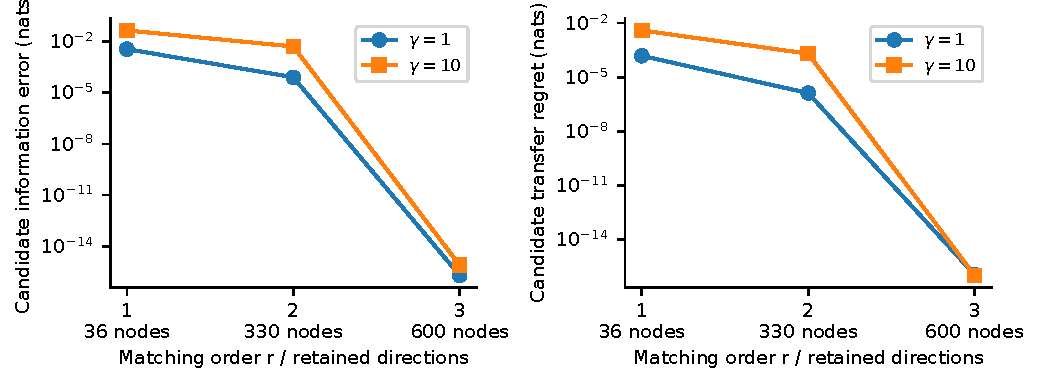
\includegraphics[width=0.95\textwidth]{figures/fig_rank_transfer.pdf}
\caption{Eight-dimensional rank-two design transfer over a common finite candidate family. Orders one and two use compressed laws; order three retains the original 600-direction law. Values below $10^{-16}$ are displayed at that floor. The curves do not certify optimization over all rank-two projectors.}
\label{fig:rank_transfer}
\end{figure}


\subsection{Auxiliary Reference Checks}
The accompanying auxiliary computation checks real and complex Haar coverage using $60000$ normalized Gaussian directions for each of $(d,K)=(3,1),(8,2),(8,4),(16,3)$. Maximum empirical Kolmogorov--Smirnov distances are $\KSReal$ and $\KSComplex$; these are sampling diagnostics. Exact finite-design curves from Proposition~\ref{prop:examples} have fitted low-SNR slopes $\SlopeAxes$ for axes/tetrahedron and $\SlopeIcosa$ for the icosahedral vertex witness. Across $1000$ random measuring directions, the latter ensemble's first two coverage moments match Haar to residual $\MomentError$.

The complex-channel normalization check is collected in Appendix~\ref{app:complex_check}.


\section{Discussion and Scope}
The eigengap and fourth-degree directional geometry play different roles. A positive eigengap gives an explicit certificate for using the leading eigenspace at finite SNR. Fourth-degree contractions determine its first displacement and the leading cubic information cost of ignoring that displacement. If the second moment is isotropic, the first-order objective is constant and fourth-degree geometry can instead select entirely different orientations, as the rotated-axis example shows.

Directional-law replacement is the statistical counterpart of measurement stability. Uniform objective approximation controls information and transferred-design regret, and a quadratic-growth condition additionally controls optimizer distance. For an unknown law, Corollary~\ref{cor:finite_sample} gives a high-probability uniform bound from independent directional samples. Classical positive cubature then compresses the empirical law while preserving the relevant even moments. At fixed dimension and bounded Gaussian SNR, the sufficient cubature support grows polynomially in the logarithm of inverse compression accuracy. The concentration term retains the usual inverse-square accuracy dependence. The constants deteriorate as the SNR interval grows, and the result is not uniform over unbounded SNR.

The Haar benchmark and covariance envelope supply reference values rather than a complete finite-SNR optimizer characterization. Haar-uniform directions make the lower benchmark exact for every fixed projector; an isotropic second moment alone does not. The upper envelope is sharp over directional laws with a prescribed second moment but can be loose for a particular law. Likewise, the stability and surrogate bounds are conservative guarantees, not predictions of typical numerical error.

The model assumes a single information-bearing amplitude and direction side information at decoding. The directional law may be known or estimated from independent direction samples, but the sampling theorem does not model the physical cost of acquiring them. The model also excludes additional front-end noise, quantization, and noncoherent decoding \cite{zhengtse2002}. The paper does not claim a computationally efficient algorithm for globally optimizing the measurement projector or constructing the smallest moment-preserving surrogate. Its guarantees concern information preservation, design transfer, and optimizer stability conditional on these computational objects being available. The complex Gaussian reference is included for normalization and validation, without asserting that all real-input theorems have been extended to a complex model.

\section{Conclusion}
For coherent random rank-one signals, the scalar coverage functional yields a unified stability chain for information-optimal measurements. An explicit finite-SNR eigengap bound, a cubic covariance-design regret bound, and a fourth-moment displacement formula control measurement variation with SNR. Projective-Wasserstein and moment-based law approximation control information, transferred-design regret, and, under quadratic growth, optimizer distance; a joint bound handles simultaneous SNR and law mismatch. Independent direction samples give a high-probability uniform approximation over the continuous projector class, and the empirical law can be compressed to a finite weighted surrogate with an explicit end-to-end regret guarantee. Gaussian information admits geometric compression error in matching order at fixed finite SNR.

\appendices
\section{Proof of the Second-Order Optimal-Information Expansion}\label{app:subspace}
Work in an orthonormal eigenbasis of $S_2$ and write $U=(x^{\top},y^{\top})^{\top}$, with $x\in\R^K$ and $y\in\R^{d-K}$. For a coordinate matrix $T\in\R^{(d-K)\times K}$ near zero, a chart around $P_0$ is
\begin{equation}
W(T)=\begin{bmatrix}I_K\\T\end{bmatrix}(I_K+T^{\top}T)^{-1/2},\quad
P(T)=W(T)W(T)^{\top}.
\end{equation}
Set $D_{ji}=\lambda_i-\lambda_{K+j}>0$. Direct expansion gives
\begin{align}
\tr(P(T)S_2)&=a_K-\sum_{j,i}D_{ji}T_{ji}^2+O(\lVert T\rVert_F^4),\\
C_{P(T)}(U)&=\norm x^2+2y^{\top}Tx+O(\lVert T\rVert_F^2).
\end{align}
For $\gamma>0$ define $F(T,\gamma)=\I_\mu(P(T);\gamma)/\gamma$ and extend at zero using
\begin{equation}
F(T,\gamma)=\EE\!\left[C_{P(T)}(U)\int_0^1h_R'(t\gamma C_{P(T)}(U))\,dt\right].
\end{equation}
Write $\nabla_T$ for the gradient with respect to the entries of $T$. The assumed $C^3$ regularity, bounded sphere, and smooth chart make $G(T,\gamma)=\nabla_TF(T,\gamma)$ continuously differentiable (extend $h_R$ smoothly just to the left of zero). At $(T,\gamma)=(0,0)$, its derivative in $T$ is diagonal with entries $-2h_R'(0)D_{ji}$ and is invertible. The implicit-function theorem gives a unique nearby stationary branch. Let $T_\gamma$ denote the chart coordinate on this branch. The finite-SNR bound in Theorem~\ref{thm:stability}(a) places every global optimizer in this neighborhood for sufficiently small positive $\gamma$, so all such optimizers lie on this branch.

Define $A_{ji}=\EE[\norm x^2y_jx_i]$. The stationarity equation yields the explicit first displacement
\begin{equation}
(T_\gamma)_{ji}=\gamma\frac{h_R''(0)}{h_R'(0)}\frac{A_{ji}}{D_{ji}}+o(\gamma).
\label{eq:tilt}
\end{equation}
Indeed, $\partial M_2(P(T))/\partial T_{ji}|_{T=0}=4A_{ji}$. In particular, $T_\gamma=O(\gamma)$ and $\norm{P_\gamma-P_0}_F=O(\gamma)$. The leading trace changes by $O(\gamma^2)$ and $M_2$ by $O(\gamma)$, so the information value is
\begin{equation}
\I_\mu^\star(\gamma)=\gamma h_R'(0)a_K+\frac{\gamma^2h_R''(0)}2M_2(P_0)+O(\gamma^3).
\end{equation}
Formula~\eqref{eq:tilt} also identifies which fourth-degree directional contractions perturb the covariance-selected subspace.

\section{Haar Coverage Moments}
For a real Haar rank-$K$ projector and fixed unit $u$, rotate coordinates so that $u=e_1$. The vector of squared coordinates of a Haar vector has a Dirichlet distribution with parameters $(1/2,\ldots,1/2)$, meaning the simplex distribution with density proportional to $\prod_i x_i^{-1/2}$ on $x_i>0$, $\sum_i x_i=1$. The sum of the first $K$ coordinates is therefore
\begin{equation}
C\sim\operatorname{Beta}\left(\frac K2,\frac{d-K}{2}\right).
\end{equation}
Its first two moments are
\begin{equation}
\EE[C]=\frac Kd,
\qquad
\EE[C^2]=\frac{K(K+2)}{d(d+2)}.
\end{equation}
For the complex Haar case the Dirichlet parameters are all one, yielding \eqref{eq:beta_complex}.

\section{Numerical Reproduction Details}
Finite-law Gaussian expectations are direct weighted sums. In the angular search, candidate stationary points are obtained from sign changes of the derivative divided by SNR; both the search grid and the bracketing solver settings are recorded in the source. Doubling a grid is a numerical diagnostic and does not prove that all stationary points were found. The compression linear programs use the dual-simplex solver HiGHS, followed by least-squares refinement on the selected support. Saved weights, angles, and moment residuals permit independent evaluation without rerunning the solver.

Auxiliary Haar directions are normalized real or complex Gaussian vectors. Gaussian information integrals use Gauss--Jacobi nodes adapted to the Beta weight. Finite-design differences use moments $3^{-n}$ for constant coverage, $(1+5^{1-n})/6$ for an icosahedral vertex projector, and $(2n+1)^{-1}$ for real Haar coverage in $d=3,K=1$. The convergent moment series is truncated at degree $47$ for $\gamma\le0.1$ to reduce cancellation. An auxiliary angular-central-Gaussian example \cite{tyler1987} uses separate training and test samples; its achieved values and empirical covariance envelope are retained in the repository but are not used to establish optimizer displacement.

Assertions check the finite-SNR bounds in the selected examples, moment residuals, positivity and support sizes of surrogate weights, finite-design identities, and scalar information ceilings. Separate verification scripts check a three-dimensional optimizer perturbation, Gaussian reference limits, and the projective-Wasserstein and joint-stability constants on independent random cases. The repository records seeds, software versions, numerical comma-separated-value (CSV) files, and generated manuscript constants. Historical tables are isolated from these computations and are not inputs to the revision.

\section{Complex Gaussian Coverage Reference}\label{app:complex_check}
Write $\C^d$ for complex Euclidean space and $\mathcal{CN}(m,\Sigma)$ for a proper complex Gaussian law with mean $m$ and covariance $\Sigma$. For a Haar-uniform complex unit vector and a rank-$K$ complex projector,
\begin{equation}
C\sim\operatorname{Beta}(K,d-K).
\label{eq:beta_complex}
\end{equation}
For the proper complex model $Y=\sqrt\gamma UR+N$, with $R\sim\mathcal{CN}(0,1)$ and $N\sim\mathcal{CN}(0,I_d)$ independent, the scalar information is $\log(1+s)$, without the real factor $1/2$. Accordingly, the Haar-averaged information is $\EE\log(1+\gamma C)$ and its high-SNR loss tends to $\psi(d)-\psi(K)$. We use the complex model as a short normalization check rather than as a second main theorem system.

\section*{Code Availability}
The source code, numerical data, and scripts used to generate the figures are available at
\url{https://github.com/HuyHoangLe0201/stability-fixed-subspace-measurements}.

\begin{thebibliography}{99}

\bibitem{prelov2004}
V. V. Prelov and S. Verd\'u, ``Second-order asymptotics of mutual information,'' \emph{IEEE Trans. Inf. Theory}, vol. 50, no. 8, pp. 1567--1580, Aug. 2004, doi: 10.1109/TIT.2004.831784.

\bibitem{verdu2002}
S. Verd\'u, ``Spectral efficiency in the wideband regime,'' \emph{IEEE Trans. Inf. Theory}, vol. 48, no. 6, pp. 1319--1343, June 2002, doi: 10.1109/TIT.2002.1003824.

\bibitem{guo2005}
D. Guo, S. Shamai, and S. Verdú, ``Mutual information and minimum mean-square error in Gaussian channels,'' \emph{IEEE Trans. Inf. Theory}, vol. 51, no. 4, pp. 1261--1282, Apr. 2005, doi: 10.1109/TIT.2005.844072.

\bibitem{guo2011}
D. Guo, Y. Wu, S. Shamai, and S. Verd\'u, ``Estimation in Gaussian noise: Properties of the minimum mean-square error,'' \emph{IEEE Trans. Inf. Theory}, vol. 57, no. 4, pp. 2371--2385, Apr. 2011, doi: 10.1109/TIT.2011.2111010.

\bibitem{palomar2006}
D. P. Palomar and S. Verdú, ``Gradient of mutual information in linear vector Gaussian channels,'' \emph{IEEE Trans. Inf. Theory}, vol. 52, no. 1, pp. 141--154, Jan. 2006, doi: 10.1109/TIT.2005.860424.

\bibitem{payaro2009}
M. Payaró and D. P. Palomar, ``Hessian and concavity of mutual information, differential entropy, and entropy power in linear vector Gaussian channels,'' \emph{IEEE Trans. Inf. Theory}, vol. 55, no. 8, pp. 3613--3628, Aug. 2009, doi: 10.1109/TIT.2009.2023749.

\bibitem{ramos2014}
A. G. C. P. Ramos and M. R. D. Rodrigues, ``Fading channels with arbitrary inputs: Asymptotics of the constrained capacity and information and estimation measures,'' \emph{IEEE Trans. Inf. Theory}, vol. 60, no. 9, pp. 5653--5672, Sept. 2014, doi: 10.1109/TIT.2014.2333746.

\bibitem{carson2013}
W. R. Carson, M. Chen, M. R. D. Rodrigues, R. Calderbank, and L. Carin, ``Communications-inspired projection design with application to compressive sensing,'' \emph{SIAM J. Imaging Sci.}, vol. 5, no. 4, pp. 1185--1212, 2012, doi: 10.1137/120878380.

\bibitem{wang2017}
L. Wang, M. Chen, M. R. D. Rodrigues, D. Wilcox, R. Calderbank, and L. Carin, ``Information-theoretic compressive measurement design,'' \emph{IEEE Trans. Pattern Anal. Mach. Intell.}, vol. 39, no. 6, pp. 1150--1164, June 2017, doi: 10.1109/TPAMI.2016.2568189.

\bibitem{goisaac2022}
J. Go and T. Isaac, ``Robust expected information gain for optimal Bayesian experimental design using ambiguity sets,'' in \emph{Proc. 38th Conf. Uncertainty in Artificial Intelligence}, ser. Proc. Mach. Learn. Res., vol. 180, 2022, pp. 728--737.

\bibitem{giraldi2018}
L. Giraldi, O. P. Le Maître, I. Hoteit, and O. M. Knio, ``Optimal projection of observations in a Bayesian setting,'' \emph{Comput. Statist. Data Anal.}, vol. 124, pp. 252--276, Aug. 2018, doi: 10.1016/j.csda.2018.03.002.

\bibitem{chechik2005}
G. Chechik, A. Globerson, N. Tishby, and Y. Weiss, ``Information bottleneck for Gaussian variables,'' \emph{J. Mach. Learn. Res.}, vol. 6, pp. 165--188, 2005.

\bibitem{li2026}
F. Li, R. Baptista, and Y. Marzouk, ``Expected information gain estimation via density approximations: Sample allocation and dimension reduction,'' \emph{SIAM/ASA J. Uncertainty Quantif.}, vol. 14, no. 3, pp. 974--1007, 2026, doi: 10.1137/25M1740164.

\bibitem{lu2007}
Y.-E. Lu, P. Liò, and S. Hand, ``Beta random projection,'' in \emph{Proc. Ninth IEEE Int. Symp. Multimedia Workshops (ISMW)}, 2007, pp. 323--328, doi: 10.1109/ISM.Workshops.2007.61.

\bibitem{kang2024}
S. Kang and H.-S. Oh, ``Spherical random projection,'' \emph{J. Roy. Statist. Soc. Ser. B}, vol. 86, no. 5, pp. 1364--1382, Nov. 2024, doi: 10.1093/jrsssb/qkae035.

\bibitem{love2003}
D. J. Love, R. W. Heath, Jr., and T. Strohmer, ``Grassmannian beamforming for multiple-input multiple-output wireless systems,'' \emph{IEEE Trans. Inf. Theory}, vol. 49, no. 10, pp. 2735--2747, Oct. 2003, doi: 10.1109/TIT.2003.817466.

\bibitem{dai2008}
W. Dai, Y. Liu, and B. Rider, ``Quantization bounds on Grassmann manifolds and applications to MIMO communications,'' \emph{IEEE Trans. Inf. Theory}, vol. 54, no. 3, pp. 1108--1123, Mar. 2008, doi: 10.1109/TIT.2007.915691.

\bibitem{delsarte1977}
P. Delsarte, J. M. Goethals, and J. J. Seidel, ``Spherical codes and designs,'' \emph{Geometriae Dedicata}, vol. 6, no. 3, pp. 363--388, 1977, doi: 10.1007/BF03187604.

\bibitem{reznick1995}
B. Reznick, ``Some constructions of spherical 5-designs,'' \emph{Linear Algebra Appl.}, vol. 226--228, pp. 163--196, 1995, doi: 10.1016/0024-3795(95)00101-V.

\bibitem{hughes2021}
D. Hughes and S. Waldron, ``Spherical $(t,t)$-designs with a small number of vectors,'' \emph{Linear Algebra Appl.}, vol. 608, pp. 84--106, Jan. 2021, doi: 10.1016/j.laa.2020.08.010.

\bibitem{bayer2006}
C. Bayer and J. Teichmann, ``The proof of Tchakaloff's theorem,'' \emph{Proc. Amer. Math. Soc.}, vol. 134, no. 10, pp. 3035--3040, 2006, doi: 10.1090/S0002-9939-06-08249-9.

\bibitem{hoeffding1963}
W. Hoeffding, ``Probability inequalities for sums of bounded random variables,'' \emph{J. Amer. Statist. Assoc.}, vol. 58, no. 301, pp. 13--30, 1963, doi: 10.1080/01621459.1963.10500830.

\bibitem{zhengtse2002}
L. Zheng and D. N. C. Tse, ``Communication on the Grassmann manifold: A geometric approach to the noncoherent multiple-antenna channel,'' \emph{IEEE Trans. Inf. Theory}, vol. 48, no. 2, pp. 359--383, Feb. 2002, doi: 10.1109/18.978730.

\bibitem{tyler1987}
D. E. Tyler, ``Statistical analysis for the angular central Gaussian distribution on the sphere,'' \emph{Biometrika}, vol. 74, no. 3, pp. 579--589, Sept. 1987, doi: 10.1093/biomet/74.3.579.

\end{thebibliography}

\end{document}
